% INFORME GR09: TODO EL TEXTO ESTA EN ESTE ARCHIVO.
% Ubicacion: informe/informe_tarea2.tex dentro del repositorio.
% Figuras de resultados P: figuras_P/. Figuras analiticas de main: figuras_diseno/.
% Buscar PENDIENTE para localizar el cierre del integrante 3 y las validaciones restantes.
% No se usan archivos externos de texto ni una carpeta secciones/.
\documentclass[journal,twocolumn]{IEEEtran}
\usepackage[utf8]{inputenc}
\usepackage[T1]{fontenc}
\usepackage[provide=*,spanish]{babel}
\usepackage{amsmath,amssymb,booktabs,graphicx,tikz,xurl,flafter,tabularx,array}
\addto\captionsspanish{\renewcommand{\figurename}{Figura}\renewcommand{\tablename}{Tabla}}
\graphicspath{{figuras_P/}{figuras_diseno/}}
\setlength{\emergencystretch}{1em}

\begin{document}

\title{Control de temperatura de una celda Peltier: análisis proporcional y diseño de un compensador PI con anti-windup}
\author{Carlos Andrés Castro Villegas, Victoria Slyn Cerdas López y Jiahui Zhong Xie%
\thanks{Escuela de Ingeniería Electrónica, Instituto Tecnológico de Costa Rica. EI-4419 Análisis y Control de Sistemas Lineales, Grupo 9, II semestre de 2026.}}
\maketitle

\begin{abstract}
Se estudia el control de la temperatura del bloque frío de la planta Peltier de la Tarea 1. Se implementa un controlador proporcional con sesgo de equilibrio y corriente limitada entre 0 y 2 A. Se comparan una planta lineal y una red física de Simscape mediante 27 ensayos de referencia, arranque, perturbaciones y ruido. También se evalúan seis condiciones de sensibilidad. Los resultados muestran que aumentar la ganancia reduce el error residual y el tiempo de arranque, pero amplifica las fluctuaciones de corriente y temperatura. La capacidad de disipación limita las referencias alcanzables y debe distinguirse del desempeño del controlador.
Se incorpora el diseño PI de la integrante 2, con $K_c=0.75\,\mathrm{A/K}$, $T_i=116.2\,\mathrm s$ e integración condicional. Sus predicciones lineales ideales y la prueba auxiliar de arranque se distinguen de los ensayos P ejecutados. \textit{PENDIENTE, integrante 3: cerrar el resumen con la validación del PI en Simscape y la comparación final.}
\end{abstract}

\begin{IEEEkeywords}
Celda Peltier, control proporcional, regulación térmica, Simscape, sensibilidad paramétrica, controlador PI.
\end{IEEEkeywords}

% ================================================================
% INTEGRANTE 3: COMPLETAR ESTA SECCION.
% ================================================================
\section{Introducción}
\textit{PENDIENTE, integrante 3: contexto de la aplicación, objetivo del proyecto y relación con la Tarea 1.}

% ================================================================
% INTEGRANTE 3: COMPLETAR ESTAS DOS SUBSECCIONES.
% ================================================================
\section{Descripción del sistema y modelo de la planta}
\subsection{Sistema físico}
\textit{PENDIENTE, integrante 3: describir la celda, el bloque frío, el disipador, el ventilador y el sensor. Agregar la tabla de parámetros con sus fuentes y un diagrama funcional.}

\subsection{Modelo de la Tarea 1}
\textit{PENDIENTE, integrante 3: resumir los balances no lineales, el espacio de estados y las hipótesis de la Tarea 1. Incorporar una imagen legible de la red Simscape. La función de transferencia usada en el análisis P aparece en la ecuación~\eqref{eq:G}.}

% ================================================================
% INTEGRANTE 1: IMPLEMENTACION DEL LAZO P.
% ================================================================
\section{Implementación del lazo cerrado}\label{sec:lazo}
\subsection{Variable controlada y referencia}
Se conserva la planta de la Tarea 1: la entrada es la corriente de la celda y la salida es la temperatura $T_b$ del bloque frío. La referencia nominal es $5\,^{\circ}\mathrm C$, con ambiente de $25\,^{\circ}\mathrm C$ y ventilación de $400\,\mathrm{LFM}$. El archivo de parámetros del grupo contiene
\begin{align}
 I_0&=1.190149\,\mathrm A, & T_{b0}&=278.15\,\mathrm K,\\
 T_{h0}&=304.101077\,\mathrm K, & R_{HA}&=1.29\,\mathrm{K/W}.
\end{align}
La regulación de temperatura es coherente con la variable física modelada. El escalón pequeño cambia la referencia de 5 a $4\,^{\circ}\mathrm C$ en $t=20\,\mathrm s$. El arranque se analiza por separado: ambas masas comienzan a $25\,^{\circ}\mathrm C$ y la referencia permanece en $5\,^{\circ}\mathrm C$. Así se distinguen seguimiento local y funcionamiento lejos del equilibrio de linealización.

\subsection{Signo del error y corriente de mando}
La planta tiene ganancia negativa alrededor del punto nominal. Se utiliza
\begin{equation}
 e_c=T_{b,\mathrm{med}}-T_{\mathrm{ref}},\qquad K_p>0,\label{eq:error_c}
\end{equation}
de manera que una temperatura excesiva aumente el esfuerzo de enfriamiento. El controlador entrega un incremento respecto de $I_0$. La corriente de mando es
\begin{equation}
 I_{\mathrm{cmd}}=\operatorname{sat}_{[0,2]}(I_0+K_p e_c).\label{eq:mando}
\end{equation}
La saturación se aplica a la corriente total, no solamente al incremento. Tanto el MAT de ensayos como su script generador usan $I_{\min}=0$ e $I_{\max}=2\,\mathrm A$.

\subsection{Límite útil de la corriente}\label{sec:limite}
El límite de $6.4\,\mathrm A$ del barrido completo de la Tarea 1 no se utiliza como límite del controlador. La curva nominal alcanza su mínimo cerca de $2.42\,\mathrm A$; aumentar la corriente por encima de esa región eleva la temperatura de equilibrio. El límite operativo de $2\,\mathrm A$ mantiene el control por debajo de ese mínimo en el caso nominal. La elección depende de la disipación, como muestra el estudio de sensibilidad.


\begin{figure}[!tbp]\centering
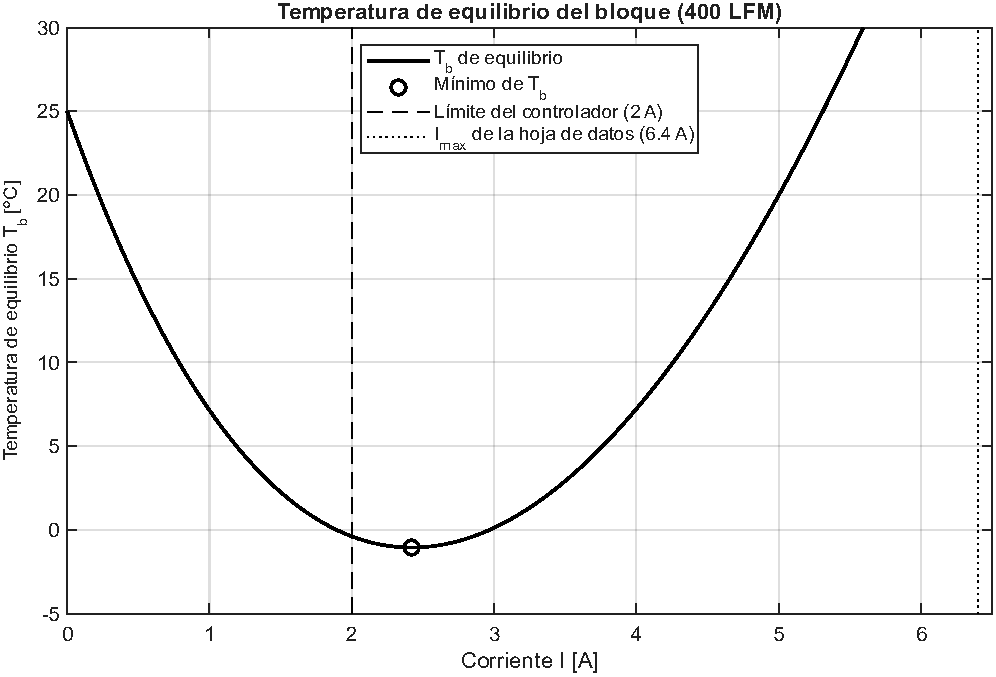
\includegraphics[width=\columnwidth]{limite_corriente.pdf}
\caption{Curva estática nominal y límite operativo de 2 A. El barrido hasta 6.4 A caracteriza la planta; no es el rango permitido del controlador. Fuente: elaboración propia a partir de la planta de la Tarea 1.}
\label{fig:limite}
\end{figure}

\subsection{Estado de corriente e interfaz Simscape}
La realimentación directa entre convertidores de la misma red física produjo avisos de lazo algebraico. Para separar el mando instantáneo de la corriente aplicada se incorporó
\begin{equation}
 \tau_I\dot I=I_{\mathrm{cmd}}-I,\qquad
 \tau_I=0.01\,\mathrm s,\qquad I(0)=I_0.\label{eq:estadoI}
\end{equation}
Para las variaciones de corriente, esta ecuación corresponde a
\begin{equation}
 H(s)=\frac{1}{0.01s+1}.\label{eq:H}
\end{equation}
El estado se implementó con un bloque \emph{State-Space}: $A=-1/\tau_I$, $B=1/\tau_I$, $C=1$ y $D=0$. Al no tener paso directo, su salida depende del estado integrado y separa el acoplamiento instantáneo de la realimentación \cite{mw_ss,mw_lim}.

Los 10 ms son una hipótesis de regularización numérica; no son una constante medida del actuador. La planta térmica de la Tarea 1 se conserva, pero la interfaz de corriente sí agrega una dinámica. Se aplicó el mismo estado en los dos modelos P. La futura comparación con el PI debe conservar esa misma condición.

En una comprobación auxiliar de las ecuaciones se estudiaron constantes de 5, 10 y 20 ms, tres ganancias P y dos pruebas: arranque y escalón. La diferencia máxima de temperatura frente a la fuente ideal fue aproximadamente 0.00232 K para 10 ms. Estos 18 casos son una verificación numérica independiente; no sustituyen los ensayos de Simscape ni validan una dinámica real del hardware.

\begin{figure}[!tbp]
\centering
\resizebox{\columnwidth}{!}{%
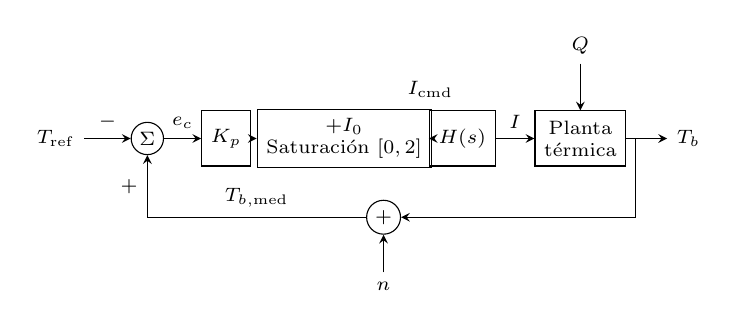
\begin{tikzpicture}[font=\scriptsize,>=stealth]
\node[draw,circle,inner sep=1.5pt] (e) at (0,0) {$\Sigma$};
\node[draw,minimum height=7mm] (kp) at (1.0,0) {$K_p$};
\node[draw,align=center,minimum height=7mm] (sat) at (2.5,0) {$+I_0$\\Saturación $[0,2]$};
\node[draw,minimum height=7mm] (h) at (4.0,0) {$H(s)$};
\node[draw,align=center,minimum height=7mm] (p) at (5.5,0) {Planta\\térmica};
\draw[->] (-0.8,0) node[left] {$T_{\mathrm{ref}}$} -- node[above] {$-$} (e);
\draw[->] (e) -- node[above] {$e_c$} (kp);
\draw[->] (kp) -- (sat);
\draw[->] (sat) -- node[above=4mm] {$I_{\mathrm{cmd}}$} (h);
\draw[->] (h) -- node[above] {$I$} (p);
\draw[->] (p) -- (6.6,0) node[right] {$T_b$};
\node[draw,circle,inner sep=1.5pt] (n) at (3.0,-1.0) {$+$};
\draw[->] (6.2,0) -- (6.2,-1.0) -- (n);
\draw[->] (3.0,-1.7) node[below] {$n$} -- (n);
\draw[->] (n) -- node[above] {$T_{b,\mathrm{med}}$} (0,-1.0) -- node[left] {$+$} (e);
\draw[->] (5.5,0.95) node[above] {$Q$} -- (p);
\end{tikzpicture}}
\caption{Lazo P implementado. La corriente aplicada es la salida del estado $H(s)$; $n$ representa ruido de medición y $Q$ una carga térmica. Fuente: elaboración propia.}
\label{fig:lazo}
\end{figure}

\subsection{Modelos e inicialización}
Se construyeron \texttt{peltier\_lazo\_P\_lineal.slx} y \texttt{peltier\_lazo\_P.slx}. El primero conserva los dos estados térmicos para representar condiciones iniciales y entradas de carga y ambiente. El segundo reutiliza la red física de la Tarea 1. La red física recibe corriente absoluta; la planta lineal recibe $\Delta I=I-I_0$. Los sensores internos se expresan en kelvin y las salidas registradas se convierten a grados Celsius. Se guardan temperatura fría y caliente, corriente, tensión y potencia eléctrica.

El script de configuración carga los parámetros en el Workspace antes de simular. Las fuentes \emph{From Workspace} mantienen el último dato después de terminar sus señales. Los constructores conectan la salida de la saturación únicamente al estado de corriente. Antes de los ensayos se comprueban las conexiones y se actualiza el diagrama; el registro recibido informa cero lazos algebraicos para ambos modelos. Los diagnósticos se mantienen activos.

\subsection{Alcance de la versión ejecutada}
Los resultados de este documento proceden del RAR ejecutado por el grupo. Los metadatos de los dos SLX nuevos indican \textbf{R2026a}. El instructivo exige R2025a, por lo que aún se debe reconstruir y repetir la comprobación final en esa versión antes de entregar. Las figuras se identifican como resultados de los archivos recibidos; no se atribuyen a una ejecución R2025a todavía no demostrada.

% ================================================================
% INTEGRANTE 1: ANALISIS TEORICO DEL CONTROL P.
% ================================================================
\section{Análisis del controlador proporcional}\label{sec:P}
\subsection{Modelo nominal y error estacionario}
La función de transferencia de corriente a temperatura alrededor del equilibrio es
\begin{equation}
G(s)=\frac{-0.291898s-0.00424337}{s^2+0.0563263s+0.000410735}.\label{eq:G}
\end{equation}
Sus polos son aproximadamente $-0.047719$ y $-0.0086074\,\mathrm{s^{-1}}$, su cero es $-0.014537\,\mathrm{s^{-1}}$ y su ganancia estática es $-10.3312\,\mathrm{K/A}$.


Para expresar el lazo con realimentación negativa se define
\begin{equation}
G_p(s)=-G(s)=\frac{0.291898s+0.00424337}{s^2+0.0563263s+0.000410735}.\label{eq:Gp}
\end{equation}

Sin saturación, la transferencia de referencia a salida, incluyendo el estado de corriente, es
\begin{equation}
T_P(s)=\frac{-K_pH(s)G(s)}{1-K_pH(s)G(s)}.
\end{equation}
Como $H(0)=1$, la magnitud del error estacionario ante un cambio de referencia de magnitud $|\Delta r|$ es
\begin{equation}
 |e_{ss}|=\frac{|\Delta r|}{1+10.3312K_p}.\label{eq:ess}
\end{equation}
Para un escalón de 1 K, las predicciones lineales son 0.32613, 0.08825 y 0.01899 K para $K_p=0.2$, 1 y $5\,\mathrm{A/K}$. El aumento de ganancia reduce el error, pero no lo elimina para una ganancia finita.

Esto no implica que el arranque deba terminar con ese mismo error. El arranque retorna al punto nominal para el cual $I_0$ ya equilibra las pérdidas térmicas. Por ello, si el sistema converge sin una perturbación permanente, el sesgo puede permitir error final prácticamente nulo.

\subsection{Polos y alcance de la estabilidad}
Con fuente ideal, el polinomio característico es
\begin{align}
D_0(s)&=s^2+(0.0563263+0.291898K_p)s\notag\\
&\quad+0.000410735+0.00424337K_p.\label{eq:carP}
\end{align}
Sus coeficientes positivos permiten concluir estabilidad del modelo ideal de segundo orden para $K_p>0$. Con el estado de corriente, el polinomio es de tercer orden:
\begin{align}
D_H(s)&=(0.01s+1)(s^2+0.0563263s+0.000410735)\notag\\
&\quad+K_p(0.291898s+0.00424337).
\end{align}
La Tabla~\ref{tab:polos} presenta los polos calculados para las tres ganancias ensayadas. Todos tienen parte real negativa. Esta comprobación lineal no demuestra estabilidad global de la planta no lineal saturada ni regulación con cualquier disipador.

\begin{table}[!tbp]\centering
\caption{Polos del modelo P con estado de corriente, sin saturación.}
\label{tab:polos}
\footnotesize
\begin{tabular}{@{}rrrr@{}}\toprule
$K_p$ [A/K] & $p_1$ [s$^{-1}$] & $p_2$ [s$^{-1}$] & $p_3$ [s$^{-1}$]\\\midrule
0.2 & -99.9416 & -0.10247 & -0.01230 \\
1.0 & -99.7071 & -0.33528 & -0.01392 \\
5.0 & -98.5179 & -1.52400 & -0.01440 \\
\bottomrule\end{tabular}
\end{table}


\subsection{Respaldo analítico ideal}
La Figura~\ref{fig:lgrP} presenta el lugar de las raíces de $K_pG_p(s)$ calculado para fuente ideal, $H(s)=1$. Una rama se aproxima al cero de la planta y otra avanza hacia valores más negativos. La posición de los polos y el peso de cada modo deben examinarse conjuntamente: una subida rápida no excluye una cola lenta.
\begin{figure}[!tbp]\centering
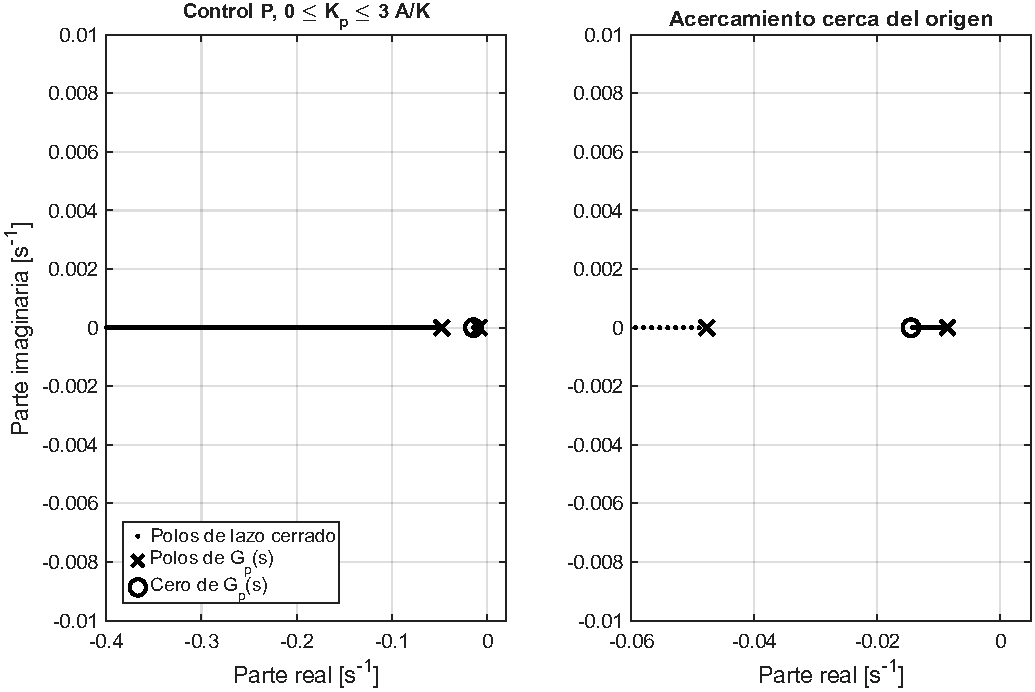
\includegraphics[width=\columnwidth]{lgr_P.pdf}
\caption{Lugar de las raíces P del modelo ideal. No incluye el polo de 10 ms de la implementación actual. Fuente: elaboración propia.}
\label{fig:lgrP}
\end{figure}
Los balances térmicos del diseño definen $G_d(s)=\Delta T_b/\Delta T_{\rm amb}$ y $G_q(s)=\Delta T_b/Q$. Sus ganancias estáticas son aproximadamente 0.918 K/K y 2.51 K/W. En ausencia de saturación permanente se obtiene
\begin{align}
\Delta T_{b,ss}^{(\rm amb)}&=\frac{4.59\,\mathrm K}{1+10.33K_p},\notag\\
\Delta T_{b,ss}^{(Q)}&=\frac{5.02\,\mathrm K}{1+10.33K_p}.\label{eq:essD}
\end{align}
La Tabla~\ref{tab:P_analitico} presenta el barrido analítico ideal de cinco ganancias. Sus tiempos se calculan con \texttt{stepinfo} respecto del valor final alcanzado; no se sustituyen por los tiempos a referencia de la Tabla~\ref{tab:escalon}. El estado $H(s)$ tiene ganancia DC unitaria, pero modifica la dinámica y los polos.
\begin{table*}[!tbp]\centering
\caption{Desempeño lineal ideal del control P, sin saturación (escalón de referencia de $1\,\mathrm K$, $+5\,\mathrm K$ en $T_{\rm amb}$ y carga de $2\,\mathrm W$).}\label{tab:P_analitico}
{\footnotesize\setlength{\tabcolsep}{3pt}\renewcommand{\arraystretch}{1.15}\setlength{\tabcolsep}{2.2pt}
\begin{tabular}{@{}ccccccc@{}}\toprule
\shortstack{$K_p$\\{[A/K]}} & \shortstack{$e_{ss}$\\{[\%]}} & \shortstack{$t_s$ (2\,\%)\\{[s]}} & \shortstack{$\Delta I_{\max}$\\{[A]}} & \shortstack{$\Delta T_{b,ss}$\\$T_{\rm amb}$ [K]} & \shortstack{$\Delta T_{b,ss}$\\2\,W [K]} & \shortstack{Polos\\{[$\mathrm{s^{-1}}$]}}\\\midrule
0.2 & 32.6 & 176.5 & 0.20 & 1.497 & 1.636 & $-0.1024$, $-0.0123$\\
0.5 & 16.2 & 106.7 & 0.50 & 0.744 & 0.813 & $-0.1889$, $-0.0134$\\
1.0 & 8.8 & 57.0 & 1.00 & 0.405 & 0.443 & $-0.3343$, $-0.0139$\\
2.0 & 4.6 & 11.5 & 2.00 & 0.212 & 0.232 & $-0.6259$, $-0.0142$\\
5.0 & 1.9 & 3.0 & 5.00 & 0.087 & 0.095 & $-1.5014$, $-0.0144$\\\bottomrule
\end{tabular}}
\par\smallskip\footnotesize Fuente: elaboración propia con \texttt{diseno\_compensador.m}, $H(s)=1$.
\end{table*}


\subsection{Esfuerzo inicial y saturación}
En el arranque, el error inicial del controlador es 20 K. Antes de limitar, la corriente solicitada es $I_0+20K_p$: aproximadamente 5.19, 21.19 y 101.19 A. Los tres valores exceden 2 A, por lo que todos los mandos arrancan saturados. La corriente aplicada inicia en $I_0$ y evoluciona según la ecuación~\eqref{eq:estadoI}; no debe confundirse con un salto instantáneo del mando.

En el escalón de $-1$ K, las ganancias de 1 y $5\,\mathrm{A/K}$ también alcanzan el límite durante el transitorio. El límite protege el rango de operación, pero impide interpretar esos tramos como una respuesta lineal sin saturación. Se distinguen la corriente total $I$ y el incremento $\Delta I=I-I_0$.

% ================================================================
% INTEGRANTE 1: METRICAS, ENSAYOS Y RESULTADOS REALES.
% ================================================================
\section{Evaluación del desempeño proporcional}\label{sec:resultadosP}
\subsection{Condiciones de los ensayos}
Las tablas se elaboran a partir de \texttt{analisis\_P.csv}, \texttt{metricas\_P.csv} y \texttt{sensibilidad\_P.csv}, conservados en \texttt{resultados\_matlab/}. Las figuras proceden de esa misma ejecución.

Cada simulación dura 1200 s y se registra con paso de salida de 0.2 s. Se usan $K_p=0.2$, 1 y $5\,\mathrm{A/K}$. Escalón, arranque, carga y ruido se repiten en ambas plantas; el cambio de ambiente se aplica solo a la planta lineal. Esto produce 27 ensayos: 24 comunes y tres de ambiente.

La carga aporta 2 W al bloque frío desde $t=300$ s. El ruido de medición comienza en ese mismo instante, en un ensayo separado; tiene desviación estándar elegida de 0.05 K, período de actualización de 1 s y semilla 9. Se utiliza la misma realización para comparar ganancias y plantas. Esta señal representa una condición de prueba, no la calibración de un sensor real.

\subsection{Definición e interpretación de las métricas}
La función \texttt{metricas\_lazo.m} utiliza el error de seguimiento $e_r=T_{\mathrm{ref}}-T_b$. Su signo es opuesto al del error del controlador, por lo que las tablas presentan principalmente $|e_{ss}|$. Se calculan
\begin{equation}
\mathrm{ISE}=\int_{t_i}^{t_f}e_r^2(t)\,dt,
\qquad \Delta I_{\max}=\max |I-I_0|.
\end{equation}
El valor final se estima sobre el último 10\% del intervalo posterior al evento. Si el rango de temperatura en esa ventana supera la banda de evaluación, no se presenta el promedio como error estacionario. La prueba no constituye una demostración formal de estabilidad.

El tiempo de subida $t_r$ mide el cambio del 10 al 90\% del valor final alcanzado. Se distinguen $t_{s,\mathrm{ref}}$, permanencia dentro de la banda de la referencia, y $t_{s,\mathrm{fin}}$, estabilización alrededor del valor final estimado. En el escalón se usa una banda de 0.02 K; en el arranque, una banda de 0.4 K. También se calcula la entrada del arranque a $\pm0.5$ K y la recuperación de perturbaciones a $\pm0.1$ K.

El tiempo de saturación se aproxima integrando las muestras de corriente aplicada que están a menos de $10^{-6}$ A de un límite; su resolución depende del registro de 0.2 s. Las desviaciones de ruido se calculan sobre el último 20\% del intervalo evaluado. Cuando una métrica no se alcanza o no corresponde al ensayo se conserva como \texttt{NaN}, representada por ``--'' en las tablas. No se sustituye por cero.

\subsection{Escalón de referencia de 5 a 4 grados Celsius}
La Tabla~\ref{tab:escalon} compara el error final de ambas plantas y los tiempos de la red Simscape. Los errores lineales coinciden con la ecuación~\eqref{eq:ess}. El modelo no lineal presenta errores algo mayores, aunque mantiene la misma tendencia con la ganancia.

\begin{table}[!tbp]\centering
\caption{Escalón de $-1$ K. Tiempos Simscape medidos desde el escalón.}
\label{tab:escalon}
\footnotesize\setlength{\tabcolsep}{3pt}
\begin{tabular}{@{}rrrrrr@{}}\toprule
$K_p$ & \shortstack{$|e_{ss}|$\\lineal [K]} & \shortstack{$|e_{ss}|$\\físico [K]} & \shortstack{$t_r$\\{[s]}} & \shortstack{$t_{s,\mathrm{fin}}$\\{[s]}} & \shortstack{$t_{s,\mathrm{ref}}$\\{[s]}}\\\midrule
0.2 & 0.32613 & 0.33312 & 49.0 & 147.8 & -- \\
1.0 & 0.08825 & 0.09184 & 8.4 & 61.2 & -- \\
5.0 & 0.01899 & 0.01990 & 4.0 & 6.0 & 347.4 \\
\bottomrule\end{tabular}
\end{table}

Con $K_p=1$, el sistema se estabiliza alrededor de su valor final en 61.2 s, pero su error de 0.09184 K impide entrar permanentemente en la banda de 0.02 K de la referencia. Por eso no corresponde afirmar que sigue la referencia en 61.2 s. Con $K_p=5$, la respuesta se acerca rápido al valor final, pero la entrada a la banda de referencia ocurre a los 347.4 s; el error final de 0.01990 K está muy próximo al borde de esa banda.

No se observa sobrepaso por debajo de la referencia en estos tres ensayos. La ganancia mayor mejora el error estático, pero eleva el esfuerzo inicial y alcanza el límite de corriente. La Figura~\ref{fig:escalon} permite observar este compromiso.

\begin{figure}[!tbp]\centering
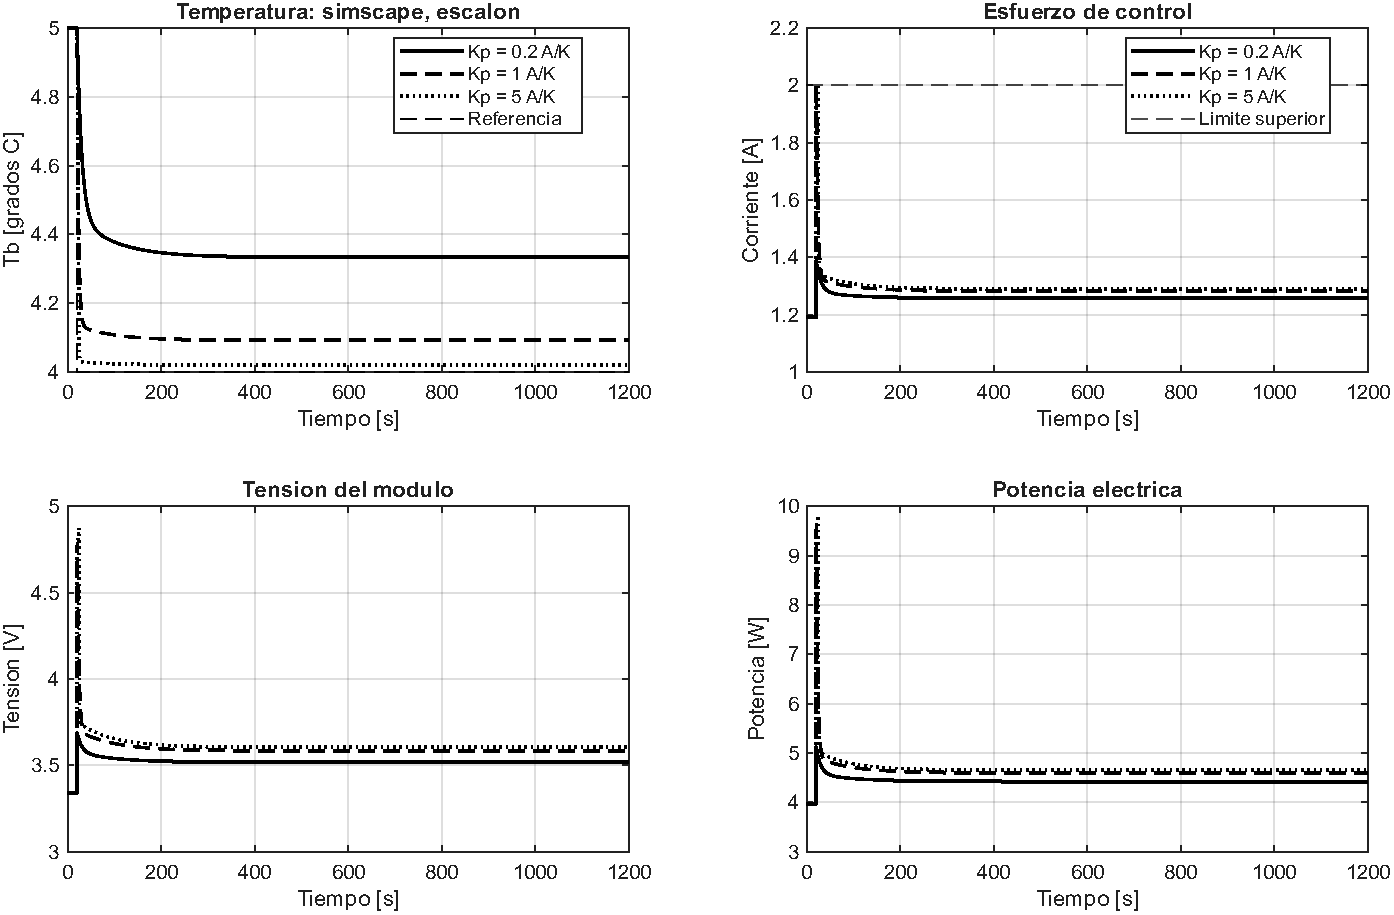
\includegraphics[width=\columnwidth]{simscape_escalon.pdf}
\caption{Escalón P en la red Simscape: temperatura, corriente, tensión y potencia. Fuente: resultados de la ejecución recibida del grupo.}
\label{fig:escalon}
\end{figure}

\subsection{Arranque desde ambiente}
Las tres ganancias llevan el bloque al entorno de 5 grados Celsius sin un descenso por debajo de la referencia en los registros. La corriente máxima es aproximadamente 2 A. La Tabla~\ref{tab:arranque} muestra que aumentar la ganancia reduce el tiempo de llegada, pero prolonga el tiempo cerca del límite de corriente.

\begin{table}[!tbp]\centering
\caption{Arranque desde 25 grados Celsius. Todas las columnas de tiempo están en segundos.}
\label{tab:arranque}
\footnotesize\setlength{\tabcolsep}{4pt}
\begin{tabular}{@{}rrrrr@{}}\toprule
$K_p$ & \shortstack{$t_s\,(\pm0.4\,\mathrm K)$\\lineal} & \shortstack{$t_s\,(\pm0.4\,\mathrm K)$\\físico} & \shortstack{$t_s\,(\pm0.5\,\mathrm K)$\\físico} & \shortstack{$t_{\mathrm{sat}}$\\físico}\\\midrule
0.2 & 217.2 & 236.8 & 218.2 & 55.4 \\
1.0 & 107.6 & 132.2 & 114.0 & 93.8 \\
5.0 & 86.6 & 101.0 & 99.2 & 105.0 \\
\bottomrule\end{tabular}
\end{table}

Para $K_p=1$, el modelo lineal predice 107.6 s frente a 132.2 s de Simscape en la banda de 0.4 K. La diferencia de 24.6 s muestra el límite de extrapolar una linealización alrededor de 5 grados Celsius a un arranque desde 25 grados Celsius. La planta física incorpora el calentamiento Joule y la evolución de la temperatura del disipador.

La temperatura caliente máxima fue aproximadamente 43.46, 43.65 y 43.65 grados Celsius para las ganancias de 0.2, 1 y 5. La mejora del arranque no debe evaluarse solo con la temperatura fría: la corriente, la potencia y la disipación también forman parte del esfuerzo requerido.

El error final cercano a cero es consistente con el sesgo $I_0$ del equilibrio nominal. El éxito del arranque no implica que el P elimine el error ante una referencia distinta o una carga permanente.

\begin{figure}[!tbp]\centering
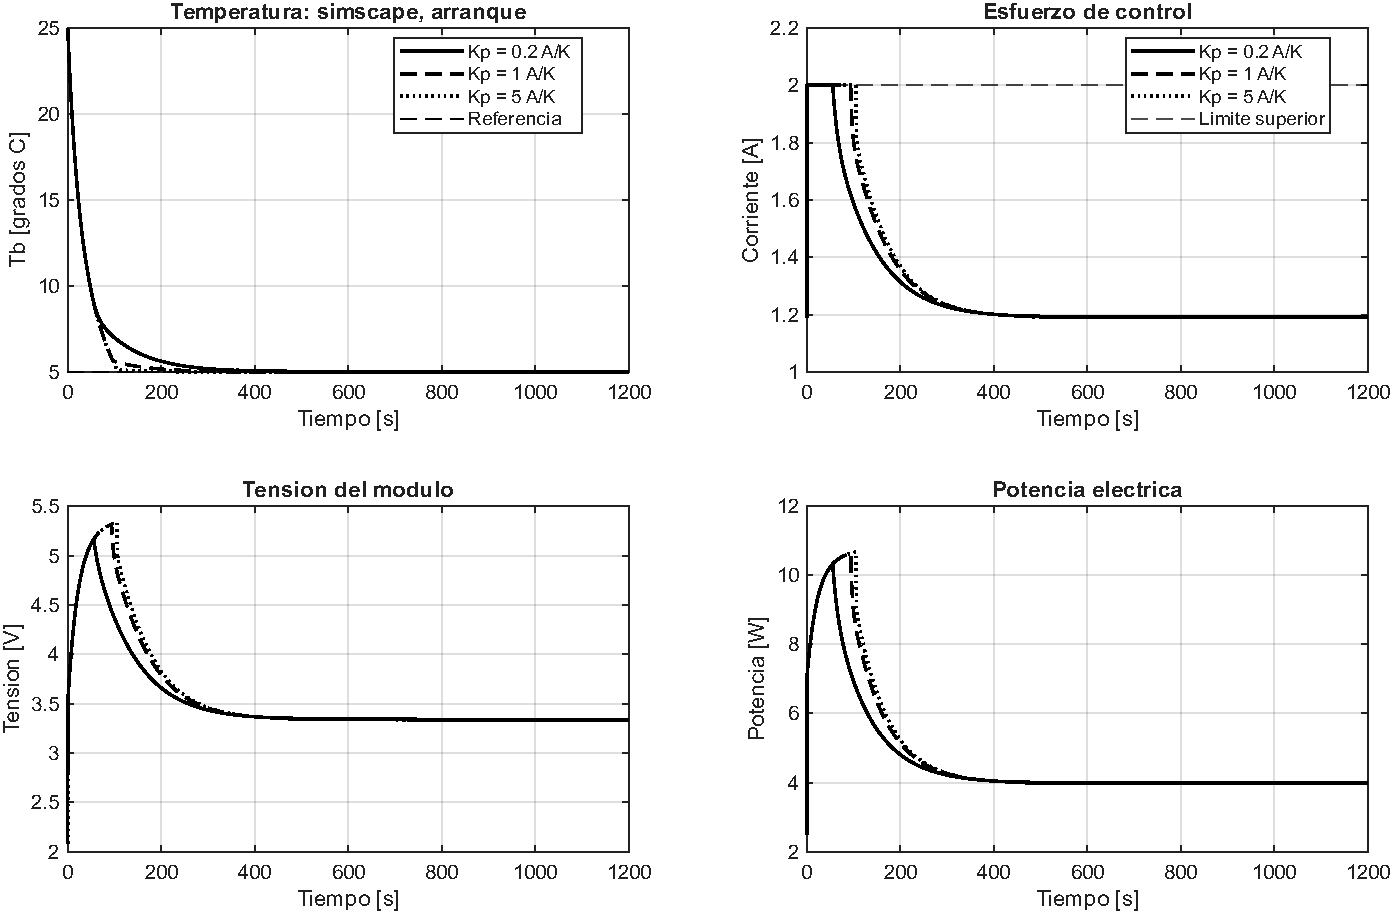
\includegraphics[width=\columnwidth]{simscape_arranque.pdf}
\caption{Arranque P desde ambiente. El mando queda limitado y la corriente aplicada sale del estado de 10 ms. Fuente: ejecución recibida del grupo.}
\label{fig:arranque}
\end{figure}

\subsection{Carga térmica y cambio de ambiente}
La carga de 2 W produce un aumento de temperatura que el P compensa parcialmente elevando la corriente. El error final disminuye con $K_p$, pero permanece distinto de cero. El cambio de ambiente de $+5$ K presenta la misma limitación en el modelo lineal. La Tabla~\ref{tab:pert} resume ambos ensayos.

\begin{table}[!tbp]\centering
\caption{Magnitud del error residual ante perturbaciones permanentes.}
\label{tab:pert}
\footnotesize
\begin{tabular}{@{}rrrr@{}}\toprule
$K_p$ & \shortstack{Carga 2 W\\lineal [K]} & \shortstack{Carga 2 W\\físico [K]} & \shortstack{Ambiente $+5$ K\\lineal [K]}\\\midrule
0.2 & 1.63549 & 1.77358 & 1.49688 \\
1.0 & 0.44258 & 0.53939 & 0.40507 \\
5.0 & 0.09524 & 0.12285 & 0.08717 \\
\bottomrule\end{tabular}
\end{table}

Una diferencia relevante aparece con $K_p=5$: la carga deja 0.09524 K en la planta lineal y 0.12285 K en Simscape. La primera predicción queda dentro de una banda de 0.1 K, mientras la segunda queda fuera. En los tres casos físicos de carga no se observa recuperación permanente a esa banda. Por tanto, la comprobación no lineal puede cambiar la evaluación del requisito de rechazo de perturbaciones.

En el ensayo lineal de ambiente, $K_p=5$ deja aproximadamente 0.08717 K. La columna de recuperación a 0.1 K toma el valor cero porque la desviación nunca sale de esa banda; esto no significa que el error final sea nulo. El control P reduce la desviación permanente, pero no la elimina.

\begin{figure}[!tbp]\centering
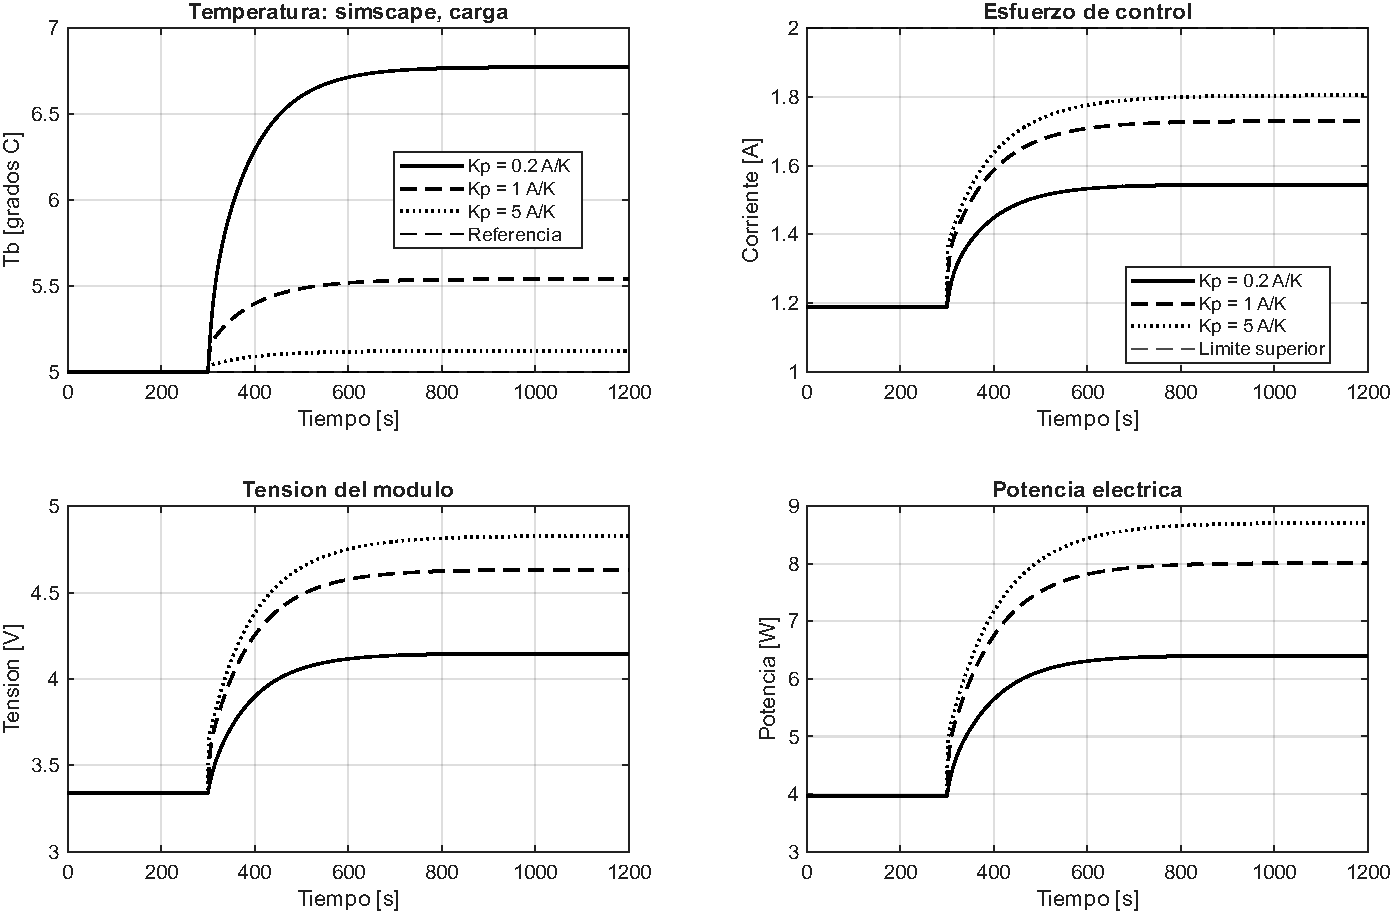
\includegraphics[width=\columnwidth]{simscape_carga.pdf}
\caption{Carga de 2 W desde 300 s en Simscape. La mayor ganancia reduce la desviación final a costa de mayor corriente. Fuente: ejecución recibida del grupo.}
\label{fig:carga}
\end{figure}

\begin{figure}[!tbp]\centering
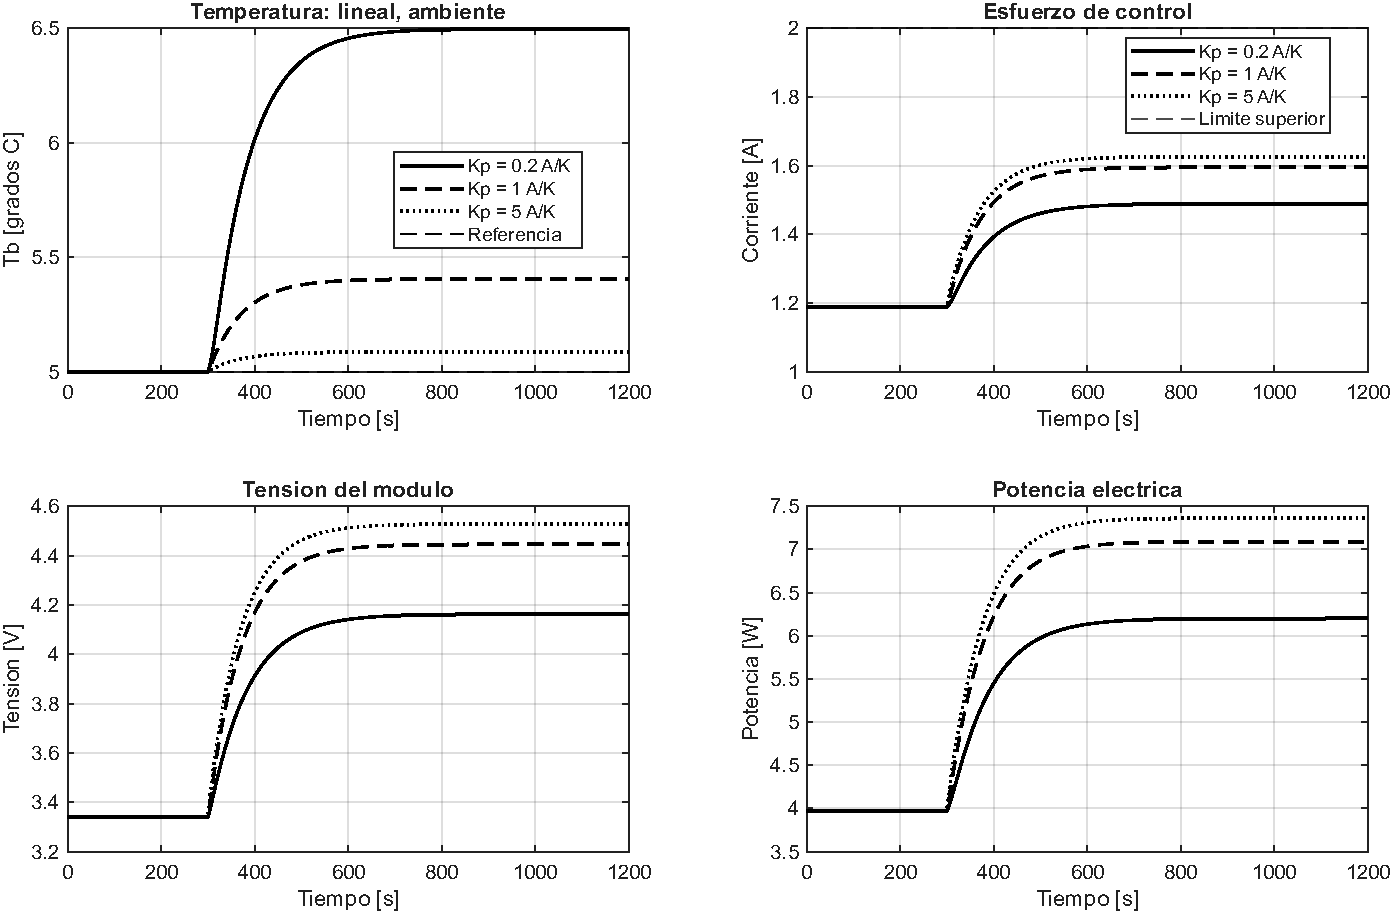
\includegraphics[width=\columnwidth]{lineal_ambiente.pdf}
\caption{Ambiente de 25 a 30 grados Celsius desde 300 s, únicamente en la planta lineal. Fuente: ejecución recibida del grupo.}
\label{fig:ambiente}
\end{figure}

\subsection{Sensibilidad al ruido de medición}
El ruido entra en la medición utilizada por el controlador; la temperatura real se conserva por separado. Los tiempos de subida y establecimiento no se interpretan en este ensayo. La Tabla~\ref{tab:ruido} presenta las fluctuaciones del tramo final y los extremos de corriente posteriores al inicio del ruido.

\begin{table}[!tbp]\centering
\caption{Ruido de medición: resultados de la planta Simscape.}
\label{tab:ruido}
\footnotesize
\begin{tabular}{@{}rrrrr@{}}\toprule
$K_p$ & $\sigma_{T_b}$ [K] & $\sigma_I$ [A] & $I_{\min}$ [A] & $I_{\max}$ [A]\\\midrule
0.2 & 0.00631 & 0.00992 & 1.153 & 1.223 \\
1.0 & 0.01865 & 0.04511 & 0.993 & 1.360 \\
5.0 & 0.03702 & 0.14915 & 0.335 & 2.000 \\
\bottomrule\end{tabular}
\end{table}

El aumento de $K_p$ eleva tanto las fluctuaciones de temperatura como las de corriente. Con $K_p=5$, la corriente alcanza brevemente el límite superior y el tiempo estimado en saturación es 0.4 s. Esto evidencia un compromiso: la ganancia que mejora el seguimiento y el rechazo de carga también transmite con mayor intensidad el ruido hacia el actuador. Las desviaciones corresponden al ruido de prueba definido, no a una garantía de exactitud física del sensor.

\begin{figure}[!tbp]\centering
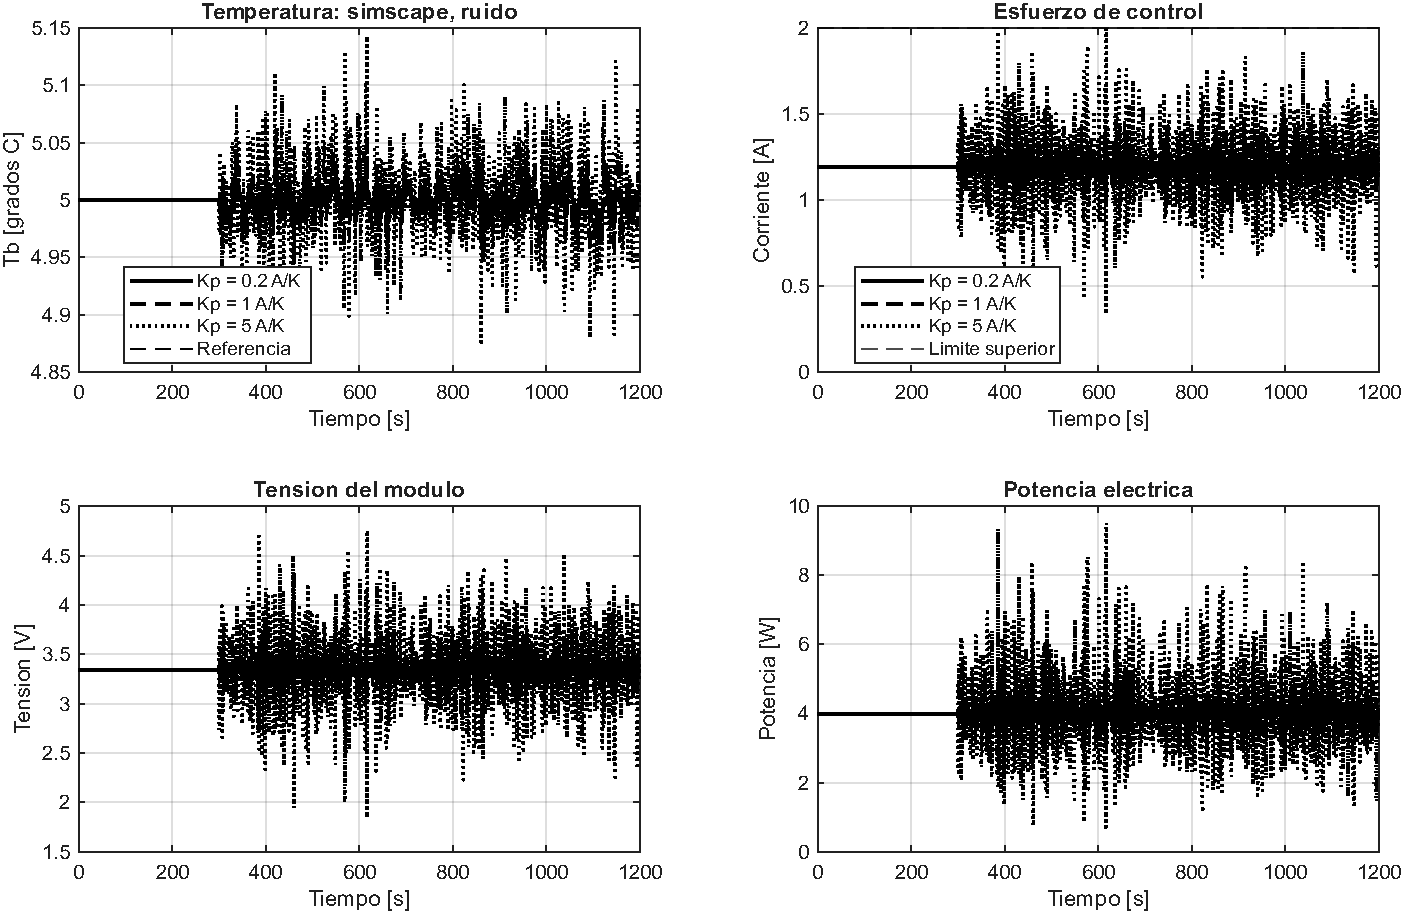
\includegraphics[width=\columnwidth]{simscape_ruido.pdf}
\caption{Respuesta P al ruido aplicado desde 300 s. Fuente: ejecución recibida del grupo.}
\label{fig:ruido}
\end{figure}

\subsection{Comprobaciones de los archivos y resultados}
Se revisaron los 27 registros P y los seis de sensibilidad: todos tienen 6001 muestras finitas hasta 1200 s. Las métricas recalculadas coinciden con las tablas entregadas. La relación eléctrica utilizada es
\begin{equation}
V=RI+\alpha(T_h-T_b),\qquad P_e=VI.
\end{equation}
La diferencia máxima observada en la primera relación fue del orden de $2\times10^{-14}$ V. Para la potencia, la diferencia frente al producto de las señales interpoladas fue menor que $10^{-4}$ W. El máximo registrado de corriente excede 2 A en aproximadamente $10^{-9}$ A, una diferencia numérica compatible con la tolerancia de la simulación.

Las figuras de resultados son PDF vectoriales. El registro contiene dos ejecuciones principales terminadas. También aparece un aviso de coincidencia de nombre del modelo lineal durante la reconstrucción; no interrumpió las ejecuciones, pero debe revisarse el path en la prueba limpia. Estas comprobaciones documentan la coherencia de los archivos recibidos; la compatibilidad final con R2025a sigue pendiente.

% ================================================================
% APORTE DE LA INTEGRANTE 2 INTEGRADO DESDE MAIN.
% ================================================================
\section{Especificaciones de diseño}\label{sec:especificaciones}
Como escenario de diseño se adopta una pequeña cámara térmica con intervalo objetivo de $+2$ a $+8\,^\circ\mathrm C$, coherente con la definición de rango aceptable del documento de equipos de conservación de vacunas de la OMS \cite{who_pqs}. La referencia de $5\,^\circ\mathrm C$ queda en su centro. Para la medición se supone un sensor digital DS18B20, con resolución de $0.0625\,^\circ\mathrm C$ en 12 bits y exactitud de $\pm0.5\,^\circ\mathrm C$ entre $-10$ y $+85\,^\circ\mathrm C$ \cite{ds18b20}. La exactitud de $\pm0.5$ grados Celsius no se confunde con la resolución ni con el error ideal de seguimiento: alcanzar 0.1 K en la simulación no garantiza esa exactitud en un equipo físico. Con este contexto se definen las especificaciones de la Tabla~\ref{tab:especificaciones}. Las especificaciones E1 a E7 se evalúan con el modelo lineal alrededor del punto de operación ($T_{b0}=5\,^\circ\mathrm C$, $I_0=1.19\,\mathrm A$); la E8 se evalúa con el modelo no lineal.

\begin{table*}[!tbp]\centering
\caption{Especificaciones de diseño del lazo de temperatura.}\label{tab:especificaciones}
{\footnotesize\setlength{\tabcolsep}{3pt}\renewcommand{\arraystretch}{1.15}
\begin{tabularx}{\textwidth}{c>{\raggedright\arraybackslash}p{3.4cm}>{\raggedright\arraybackslash}p{5.2cm}>{\raggedright\arraybackslash}X}\toprule
Id. & Métrica & Especificación & Justificación\\\midrule
E1 & Error en estado estable & $|e_{ss}|\le0.1\,\mathrm K$ para escalones de hasta $3\,\mathrm K$ & Equivale a menos de dos pasos de resolución del sensor \cite{ds18b20}. Un cambio de $3\,\mathrm K$ cubre toda la mitad del rango de $2$ a $8\,^\circ\mathrm C$ \cite{who_pqs}.\\
E2 & Sobrepaso & $M_p\le10\,\%$ & Para un escalón de $1\,\mathrm K$, el sobrepaso queda del mismo orden que la tolerancia de E1.\\
E3 & Tiempo de asentamiento (2\,\%) & $t_s\le180\,\mathrm s$ & Aproximadamente la mitad del tiempo de lazo abierto ($373\,\mathrm s$), para recuperar la temperatura después de abrir la cámara o introducir una muestra.\\
E4 & Esfuerzo de control en pequeña señal & $\Delta I_{\max}\le0.81\,\mathrm A$ ante un escalón de $-1\,\mathrm K$ & Con $I_0=1.19\,\mathrm A$, el margen positivo exacto es $2-I_0=0.809851\,\mathrm A$. El valor 0.81 A es un redondeo; además debe comprobarse que el mando no sature. La Tarea~1 mostró un error del modelo lineal cercano al $5\,\%$ con $|\Delta I|=1\,\mathrm A$.\\
E5 & Rango de la corriente & $0\le I\le2.0\,\mathrm A$ & Por debajo del mínimo de la curva estática ($2.42\,\mathrm A$, Figura~\ref{fig:limite}); la fuente no invierte la corriente.\\
E6 & Rechazo de perturbación & Escalón de $+5\,\mathrm K$ en $T_{\rm amb}$ o carga de $2\,\mathrm W$ en el bloque: pico $\le0.5\,\mathrm K$, regreso a $\pm0.1\,\mathrm K$ en $\le400\,\mathrm s$ y error final nulo & Un cambio de $25$ a $30\,^\circ\mathrm C$ en el ambiente es esperable durante el día, y la carga de $2\,\mathrm W$ representa introducir una muestra. En lazo abierto producirían $+4.6$ y $+5.0\,\mathrm K$, lo que saca al bloque del rango de $2$ a $8\,^\circ\mathrm C$.\\
E7 & Estabilidad relativa & Margen de fase $\ge45^\circ$ & Las masas del bloque y del disipador se marcaron como provisionales en la Tarea~1; el margen ofrece una reserva nominal frente a incertidumbre; no demuestra por sí solo robustez frente a cualquier variación.\\
E8 & Arranque desde $25\,^\circ\mathrm C$ (no lineal) & $T_b\ge2\,^\circ\mathrm C$ en todo momento y $|T_b-5\,^\circ\mathrm C|\le0.5\,\mathrm K$ antes de $300\,\mathrm s$ & No se aceptan temperaturas por debajo de $+2\,^\circ\mathrm C$ en el almacenamiento \cite{who_pqs}. Se exige además que el arranque sea más rápido que el de lazo abierto.\\\bottomrule
\end{tabularx}}
\par\smallskip\footnotesize Fuente: elaboración propia.
\end{table*}

Con las ecuaciones~\eqref{eq:ess} y \eqref{eq:essD} se ve que el control P no puede cumplir todas las especificaciones al mismo tiempo en el diseño lineal ideal. La E1 exige $K_p\ge2.81\,\mathrm{A/K}$ y alcanzar una desviación residual de 0.1 K en las perturbaciones de E6 exige $K_p\ge4.35\,\mathrm{A/K}$ por la temperatura ambiente y $K_p\ge4.76\,\mathrm{A/K}$ por la carga de $2\,\mathrm W$, pero la E4 limita la ganancia a $K_p\le0.81\,\mathrm{A/K}$. Ningún valor de $K_p$ satisface las tres condiciones. Además, una ganancia P finita no elimina el error permanente de E6. Se requiere una estructura con acción integral. El cumplimiento del rango completo de E1 debe contrastarse también con los límites y las pruebas de hasta $\pm3$ K, no solamente con el escalón de $-1$ K.

% Responsable: Integrante 2 (tarea 2.3 del plan)
\section{Selección del compensador}\label{sec:seleccion}
El análisis anterior identifica deficiencias de régimen permanente y rechazo de perturbaciones. También distingue una subida rápida del establecimiento a referencia: los tiempos de la Tabla~\ref{tab:escalon} no permiten descartar una limitación transitoria. En el diseño nominal ideal los polos son reales y el margen de fase calculado es amplio. La Tabla~\ref{tab:seleccion} compara las estructuras consideradas frente a estas deficiencias.

\begin{table}[!tbp]\centering
\caption{Comparación de estructuras de compensación para la planta de la ecuación~\eqref{eq:Gp}.}\label{tab:seleccion}
{\footnotesize\setlength{\tabcolsep}{3pt}\renewcommand{\arraystretch}{1.15}
\begin{tabularx}{\columnwidth}{lc>{\raggedright\arraybackslash}X}\toprule
Estructura & $e_{ss}=0$ & Comentario\\\midrule
P & No & No cumple E1, E4 y E6 a la vez (Sección~\ref{sec:especificaciones}).\\
PD / adelanto & No & Mejoran la fase y la rapidez, que no son el problema. La acción derivativa amplifica los saltos de cuantización del sensor ($0.0625\,\mathrm K$).\\
Atraso & No & Reduce el error, pero no lo anula; requiere una ganancia en DC muy alta para cumplir E6.\\
PID & Sí & Puede corregir el error estático, pero agrega una acción derivativa que aumenta complejidad y sensibilidad al ruido.\\
\textbf{PI} & \textbf{Sí} & El integrador vuelve el lazo tipo~1: error nulo ante escalones de referencia y perturbación constante, si el lazo es estable y el esfuerzo requerido es alcanzable. Es la estructura más sencilla que corrige la deficiencia observada.\\\bottomrule
\end{tabularx}}
\par\smallskip\footnotesize Fuente: elaboración propia con base en \cite{ogata}.
\end{table}

Se selecciona un controlador PI. Su efecto esperado es agregar un polo en el origen, que anula el error permanente, y un cero real que se ubica para no hacer más lento el lazo. Como la planta ya tiene un margen de fase grande, la pérdida de fase del integrador se evalúa mediante los polos y márgenes del diseño nominal.

Por la limitación de la Sección~\ref{sec:limite}, la salida del PI se satura entre $0$ y $2\,\mathrm A$. En la comprobación auxiliar de arranque el error inicial es de $20\,\mathrm K$ y la corriente pasa cerca de $100\,\mathrm s$ saturada. Si el integrador sigue acumulando error en ese tiempo (\emph{windup}), al llegar a la referencia tiene un valor excesivo y el bloque se enfría de más. Por eso el PI se implementa con anti-windup por integración condicional (\emph{clamping}): se detiene la integración cuando su evolución aumentaría el exceso de saturación y se permite descargar la integral cuando el error reduce ese exceso \cite{astrom,mw_pid}.

% Responsable: Integrante 2 (tarea 2.4 del plan)
\section{Diseño del compensador}\label{sec:diseno}
El diseño se obtuvo con fuente ideal, $H(s)=1$, y se conserva aquí como base de selección. Sus figuras y predicciones no son ensayos nuevos del PI en Simscape. La implementación final debe agregar el mismo estado de corriente de la ecuación~\eqref{eq:estadoI} que usa el P. La revisión independiente con $H(s)$ aparece en la Sección~\ref{sec:revisionPI}.
\subsection{Estructura y ley de control}
El controlador PI se escribe como
\begin{equation}
C(s)=K_c\,\frac{s+z}{s}=K_c\left(1+\frac{1}{T_is}\right),\qquad z=\frac{1}{T_i},\label{eq:PI}
\end{equation}
y la salida sin limitar del PI se expresa como
\begin{equation}
\Delta I_u=K_ce_c+x_I,\qquad \dot x_I=K_ie_c,\label{eq:ley}
\end{equation}
cuando la integración está habilitada. El anti-windup modifica la evolución de $x_I$ según la saturación. La corriente de mando total es $I_{\rm cmd}=\operatorname{sat}_{[0,2]}(I_0+\Delta I_u)$ y la corriente aplicada se obtiene del estado de 10 ms. Con $x_I(0)=0$ e $I(0)=I_0$, el sesgo y la condición inicial quedan separados del mando saturado durante el arranque.

Si el bloque PI entrega $\Delta I$, sus límites internos deben ser $[-I_0,\,2-I_0]$ A, con \emph{clamping}. Después se suma $I_0$ y se conserva el límite total de 0 a 2 A. Una saturación externa sola no informa al integrador de la limitación. La Figura~\ref{fig:lazoPI} resume la estructura prevista.

\begin{figure}[!tbp]\centering
\resizebox{\columnwidth}{!}{%
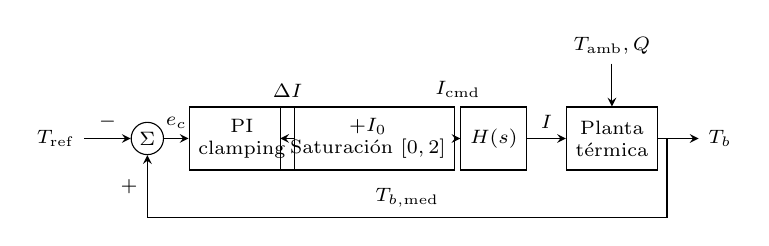
\begin{tikzpicture}[font=\scriptsize,>=stealth]
\node[draw,circle,inner sep=1.5pt] (e) at (0,0) {$\Sigma$};
\node[draw,align=center,minimum height=8mm] (pi) at (1.2,0) {PI\\clamping};
\node[draw,align=center,minimum height=8mm] (sat) at (2.8,0) {$+I_0$\\Saturación $[0,2]$};
\node[draw,minimum height=8mm] (h) at (4.4,0) {$H(s)$};
\node[draw,align=center,minimum height=8mm] (p) at (5.9,0) {Planta\\térmica};
\draw[->] (-0.8,0) node[left] {$T_{\mathrm{ref}}$} -- node[above] {$-$} (e);
\draw[->] (e) -- node[above] {$e_c$} (pi);
\draw[->] (pi) -- node[above=4mm] {$\Delta I$} (sat);
\draw[->] (sat) -- node[above=4mm] {$I_{\mathrm{cmd}}$} (h);
\draw[->] (h) -- node[above] {$I$} (p);
\draw[->] (p) -- (7.0,0) node[right] {$T_b$};
\draw[->] (6.6,0) -- (6.6,-1.0) -- node[above] {$T_{b,\mathrm{med}}$} (0,-1.0) -- node[left] {$+$} (e);
\draw[->] (5.9,0.95) node[above] {$T_{\rm amb},Q$} -- (p);
\end{tikzpicture}}
\caption{Estructura prevista del PI con límites internos de incremento de corriente, sesgo y estado de corriente. El diseño analítico original considera $H(s)=1$.}
\label{fig:lazoPI}
\end{figure}

\subsection{Ubicación del cero}
Los polos de la planta son $-0.0477$ y $-0.0086\,\mathrm{s^{-1}}$ (constantes de tiempo de $21$ y $116\,\mathrm s$). El polo lento domina la respuesta en lazo abierto. Si el integrador se agregara sin más, el polo en el origen y el polo lento formarían un par dominante muy lento. Por eso el cero del PI se coloca sobre el polo lento, de modo que lo cancele:
\begin{equation}
z=0.008607\,\mathrm{s^{-1}}\ \Rightarrow\ T_i=\frac{1}{z}=116.2\,\mathrm s.\label{eq:cero}
\end{equation}
Con esta cancelación, la ganancia de lazo abierto se reduce a
\begin{equation}
L_0(s)=C(s)G_p(s)=\frac{K_c\,(0.2919\,s+0.004243)}{s\,(s+0.04772)},\label{eq:L}
\end{equation}
y la ecuación característica del lazo cerrado queda
\begin{equation}
s^2+(0.04772+0.2919K_c)\,s+0.004243K_c=0.\label{eq:carPI}
\end{equation}
Igual que en la ecuación~\eqref{eq:carP}, todos los coeficientes son positivos para $K_c>0$, así que este modelo lineal nominal ideal es estable para $K_c>0$. Esta conclusión no se extiende automáticamente al lazo saturado ni a plantas con otros parámetros. El polo cancelado, $-0.0086\,\mathrm{s^{-1}}$, sigue presente en el lazo cerrado. No aparece en la respuesta a la referencia, pero sí en la respuesta a perturbaciones, como se discute más adelante.

\subsection{Selección de la ganancia}
Con el cero fijo, se calculó la respuesta del lazo para $0.1\le K_c\le1.5\,\mathrm{A/K}$ en pasos de $0.05$ (Figura~\ref{fig:barrido}). El tiempo de asentamiento disminuye con la ganancia y cumple la E3 a partir de $K_c=0.65\,\mathrm{A/K}$. El esfuerzo inicial vale $\Delta I(0^+)=K_c\,|\Delta T_{\rm ref}|$, por lo que la E4 limita la ganancia a $K_c\le0.81\,\mathrm{A/K}$. Dentro del intervalo $0.65\le K_c\le0.80\,\mathrm{A/K}$ el barrido ideal predice cumplimiento de los criterios lineales evaluados. Las pruebas con amplitud de hasta 3 K, límites y dinámica de corriente deben confirmarse en la implementación final. Se escoge un valor intermedio para dejar margen hacia ambos lados:
\begin{equation}
K_c=0.75\,\mathrm{A/K},\qquad K_i=\frac{K_c}{T_i}=6.456\times10^{-3}\,\mathrm{A/(K\,s)}.\label{eq:ganancias}
\end{equation}

\begin{figure}[!tbp]\centering
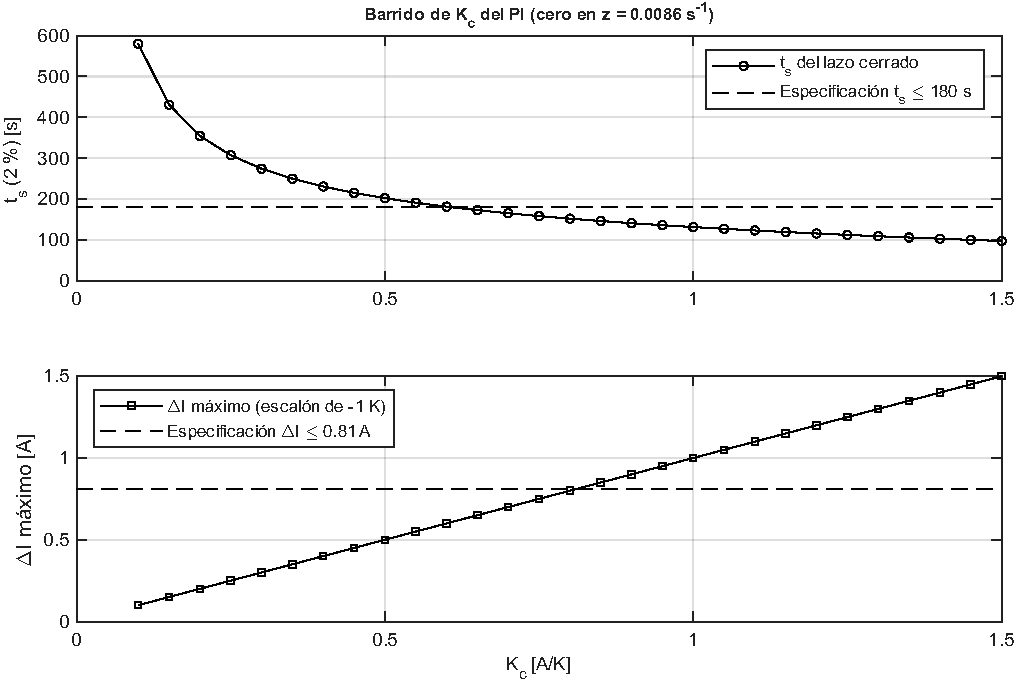
\includegraphics[width=\columnwidth]{barrido_Kc}
\caption{Tiempo de asentamiento y esfuerzo de control máximo en función de $K_c$, con el cero del PI fijo en $z=0.0086\,\mathrm{s^{-1}}$. Las líneas discontinuas son las especificaciones E3 y E4. Fuente: elaboración propia, modelo de fuente ideal.}\label{fig:barrido}
\end{figure}

Al sustituir $K_c=0.75\,\mathrm{A/K}$ en la ecuación~\eqref{eq:carPI} se obtienen los polos de lazo cerrado $-0.2541$ y $-0.0125\,\mathrm{s^{-1}}$, a los que se suma el polo cancelado en $-0.0086\,\mathrm{s^{-1}}$. La Figura~\ref{fig:lgrPI} los ubica sobre el lugar de las raíces. El polo en $-0.0125\,\mathrm{s^{-1}}$ queda muy cerca del cero en $-0.0145\,\mathrm{s^{-1}}$, por lo que su aporte a la respuesta es pequeño y la salida se acerca rápido a la referencia.

\begin{figure}[!tbp]\centering
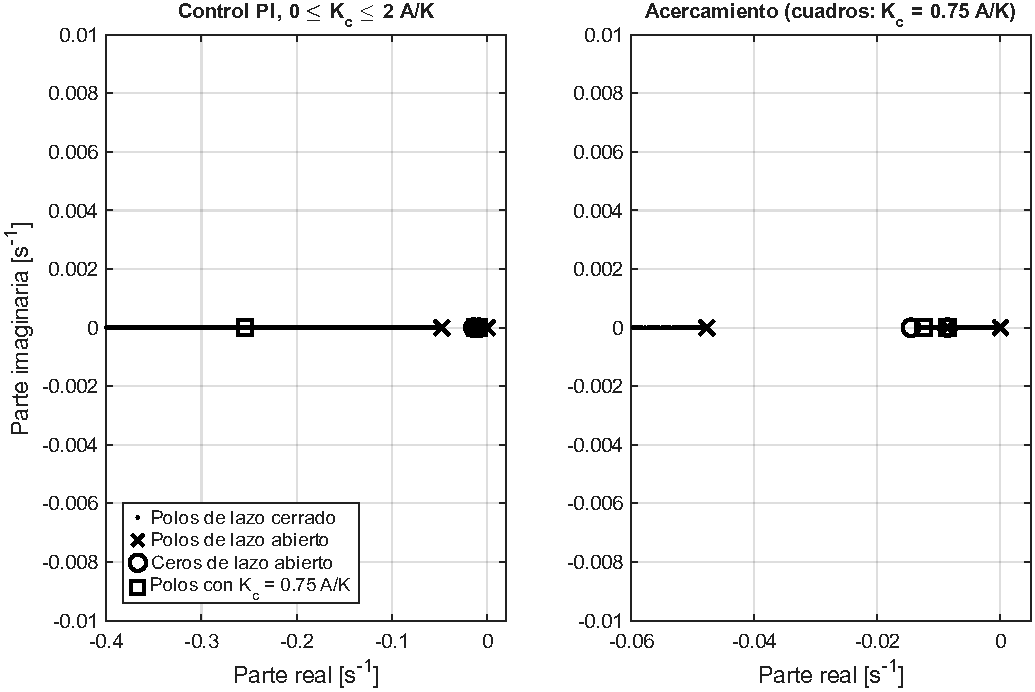
\includegraphics[width=\columnwidth]{lgr_PI}
\caption{Lugar de las raíces de $K_c(s+z)G_p(s)/s$ para $0\le K_c\le2\,\mathrm{A/K}$; los cuadrados son los polos con $K_c=0.75\,\mathrm{A/K}$. Fuente: elaboración propia, modelo de fuente ideal.}\label{fig:lgrPI}
\end{figure}

\subsection{Verificación en frecuencia}
La Figura~\ref{fig:bode} muestra el diagrama de Bode de $L_0(s)$. El margen de fase es de $98.7^\circ$ a $0.214\,\mathrm{rad/s}$ y el margen de ganancia es infinito, porque la fase nunca llega a $-180^\circ$. Se cumple la E7 con amplitud.

\begin{figure}[!tbp]\centering
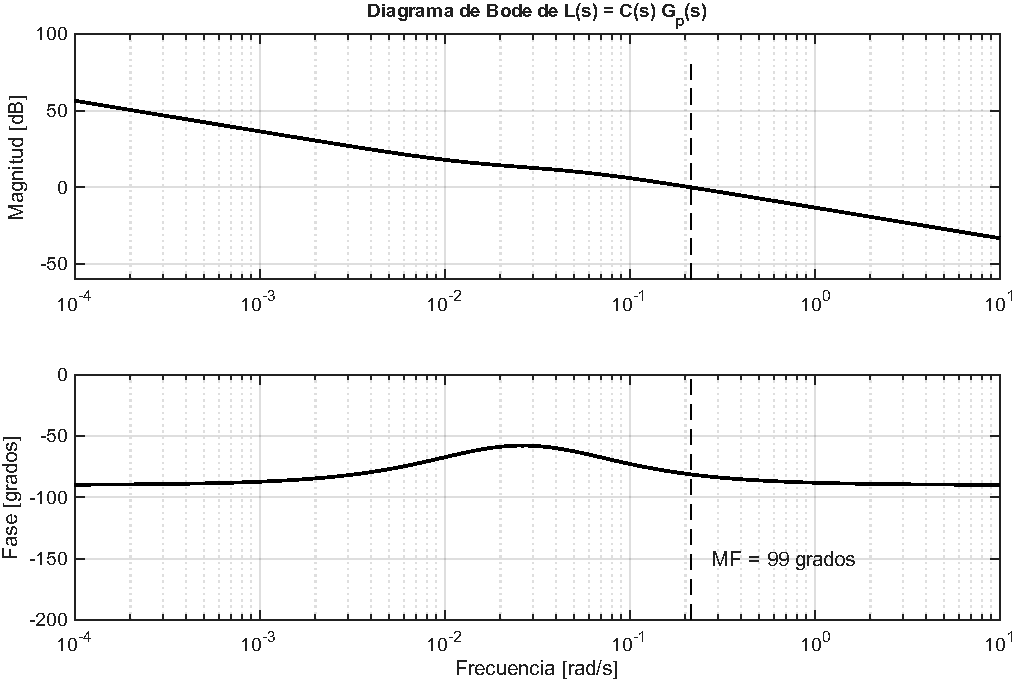
\includegraphics[width=\columnwidth]{bode_PI}
\caption{Diagrama de Bode de la ganancia de lazo $L_0(s)=C(s)G_p(s)$ con $K_c=0.75\,\mathrm{A/K}$ y $T_i=116.2\,\mathrm s$. La línea discontinua marca la frecuencia de cruce de ganancia. Fuente: elaboración propia, modelo de fuente ideal.}\label{fig:bode}
\end{figure}

\subsection{Comprobación con el modelo no lineal}
Para respaldar la elección del límite de corriente y del anti-windup se integró el modelo no lineal de la Tarea~1 con el método de Euler (paso de $0.05\,\mathrm s$) durante un arranque desde $25\,^\circ\mathrm C$ con $T_{\rm ref}=5\,^\circ\mathrm C$ (Figura~\ref{fig:arranquePIaux}). Con límite de $6.4\,\mathrm A$, la corriente se queda en el máximo y el bloque se calienta hasta $46.4\,^\circ\mathrm C$. Con límite de $2\,\mathrm A$ pero sin anti-windup, el integrador acumula error durante la saturación y el bloque baja hasta $1.92\,^\circ\mathrm C$, lo que viola la E8. Con el diseño completo, la temperatura mínima es $4.87\,^\circ\mathrm C$ y el bloque entra a la banda de $5\pm0.5\,^\circ\mathrm C$ a los $117\,\mathrm s$. La validación formal queda pendiente con la red de Simscape en la Sección~\ref{sec:resultados}.

\begin{figure}[!tbp]\centering
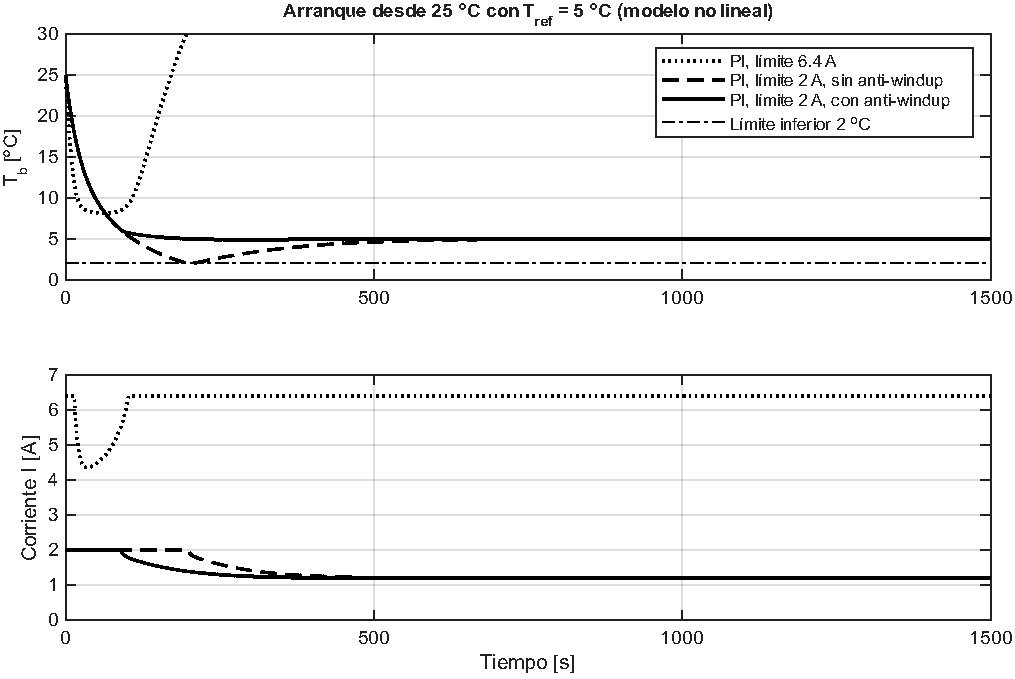
\includegraphics[width=\columnwidth]{arranque_nl}
\caption{Arranque desde $25\,^\circ\mathrm C$ con el modelo no lineal para tres implementaciones del PI ($K_c=0.75\,\mathrm{A/K}$, $T_i=116.2\,\mathrm s$). Fuente: integración auxiliar de Euler del diseño original; no es una simulación Simscape.}\label{fig:arranquePIaux}
\end{figure}

\subsection{Resumen del diseño}
La Figura~\ref{fig:escalonPPI} compara el P y el PI con la misma ganancia proporcional ($0.75\,\mathrm{A/K}$) ante un escalón de referencia de $-1\,\mathrm K$, con el modelo lineal ideal. El P se queda a $0.11\,\mathrm K$ de la referencia, mientras que el PI la alcanza; el incremento inicial solicitado es $0.75\,\mathrm A$ y la corriente total correspondiente es $I_0+0.75=1.940149\,\mathrm A$, dentro del margen previsto en E4. Estos valores de mando ideal no se confunden con $I(0)=I_0$ del estado regularizado.

\begin{figure}[!tbp]\centering
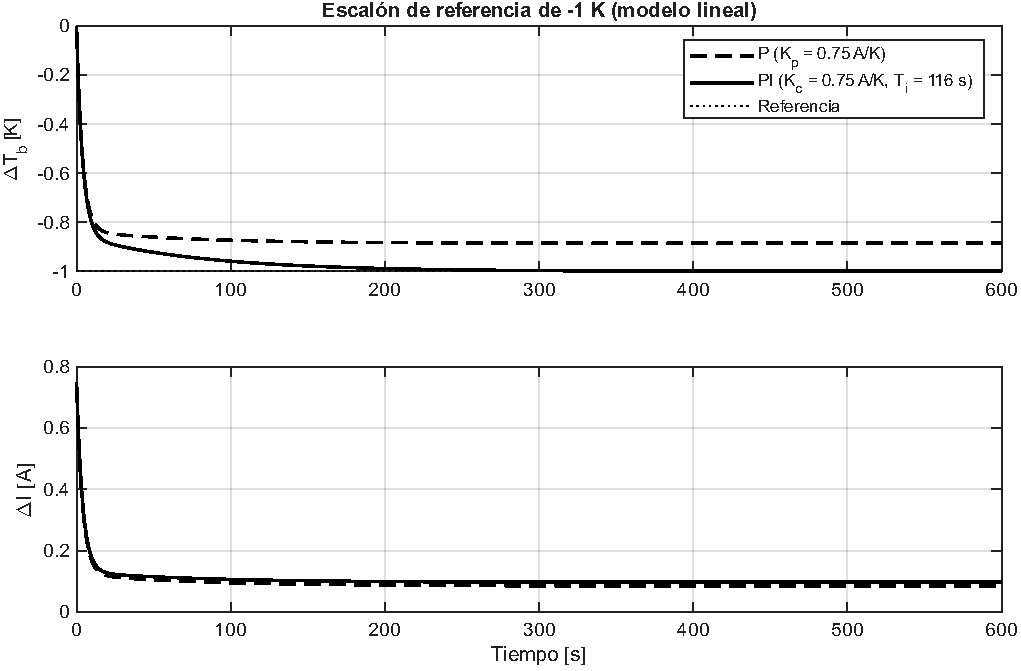
\includegraphics[width=\columnwidth]{escalon_P_PI}
\caption{Respuesta lineal a un escalón de referencia de $-1\,\mathrm K$ con control P ($K_p=0.75\,\mathrm{A/K}$) y con el PI diseñado: desviación de la temperatura (arriba) y de la corriente (abajo). Fuente: elaboración propia, modelo de fuente ideal.}\label{fig:escalonPPI}
\end{figure}

La Figura~\ref{fig:pertPPI} muestra las dos perturbaciones de la E6. En lazo abierto el bloque se desvía $4.6$ y $5.0\,\mathrm K$; con el P la desviación permanente baja a cerca de $0.5\,\mathrm K$, y con el PI el pico es de $0.26$ y $0.30\,\mathrm K$ y la desviación vuelve a cero.

\begin{figure}[!tbp]\centering
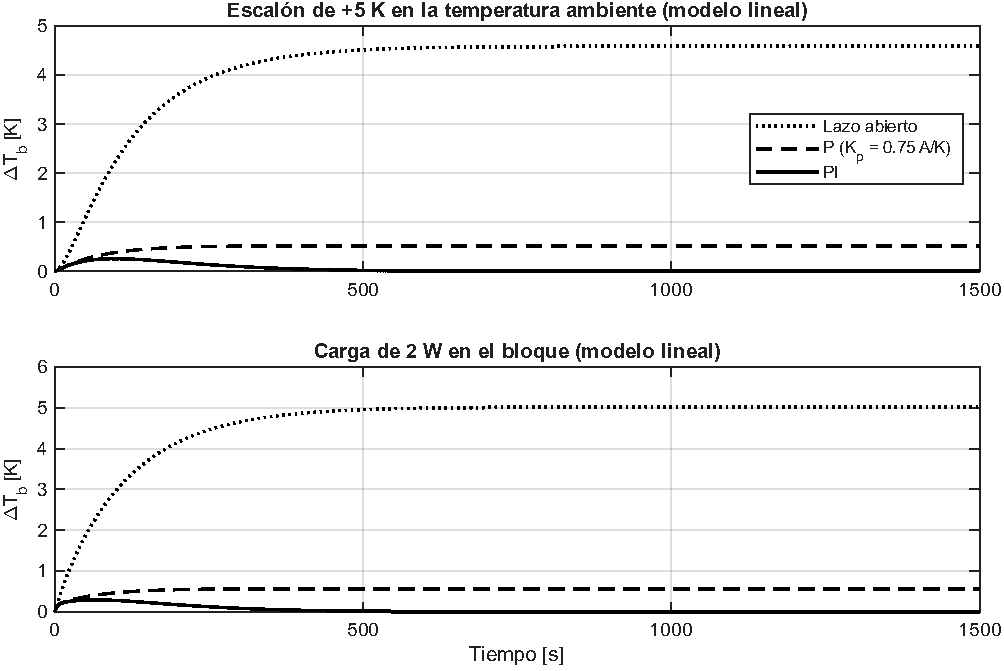
\includegraphics[width=\columnwidth]{perturbacion_P_PI}
\caption{Respuesta lineal a un escalón de $+5\,\mathrm K$ en la temperatura ambiente (arriba) y a una carga de $2\,\mathrm W$ en el bloque (abajo), en lazo abierto, con control P y con el PI. Fuente: elaboración propia, modelo de fuente ideal.}\label{fig:pertPPI}
\end{figure}

La Tabla~\ref{tab:prediccion} compara el desempeño previsto del diseño con las especificaciones de la Tabla~\ref{tab:especificaciones}. La tabla conserva los valores previstos por el diseño original; el cumplimiento final queda sujeto a los ensayos compensados y al rango completo de las especificaciones. Para la implementación en el bloque \emph{PID Controller} de Simulink se usa la forma paralela con $P=K_c$, $I=K_i$ y $D=0$, límites internos $[-I_0,2-I_0]$ en la salida de incremento y anti-windup por \emph{clamping} \cite{mw_pid}. Los valores se guardan en \texttt{parametros\_control.mat}.

\begin{table*}[!htbp]\centering
\caption{Desempeño previsto del PI frente a las especificaciones.}\label{tab:prediccion}
{\footnotesize\setlength{\tabcolsep}{3pt}\renewcommand{\arraystretch}{1.15}
\begin{tabular}{clccc}\toprule
Id. & Métrica & Especificación & PI diseñado & Etapa de comprobación\\\midrule
E1 & $e_{ss}$ & $\le0.1\,\mathrm K$ & $0$ & Ideal\\
E2 & $M_p$ & $\le10\,\%$ & $0\,\%$ & Ideal\\
E3 & $t_s$ (2\,\%) & $\le180\,\mathrm s$ & $158.6\,\mathrm s$ & Ideal\\
E4 & $\Delta I_{\max}$ ($-1\,\mathrm K$) & $\le0.81\,\mathrm A$ & $0.75\,\mathrm A$ & Ideal\\
E5 & Rango de $I$ & $0$ a $2\,\mathrm A$ & $0$ a $2\,\mathrm A$ & Limitador previsto\\
E6 & Pico / regreso & $\le0.5\,\mathrm K$ / $\le400\,\mathrm s$ & $0.30\,\mathrm K$ / $300\,\mathrm s$ & Ideal\\
E7 & Margen de fase & $\ge45^\circ$ & $98.7^\circ$ & Ideal\\
E8 & $T_{b,\min}$ / $t_{\pm0.5}$ & $\ge2\,^\circ\mathrm C$ / $\le300\,\mathrm s$ & $4.87\,^\circ\mathrm C$ / $117\,\mathrm s$ & Euler auxiliar\\\bottomrule
\end{tabular}}
\par\smallskip\footnotesize Fuente: predicciones del diseño ideal. E1 a E7 se presentan con fuente ideal y sin saturación permanente; E8 procede de Euler auxiliar. Falta confirmar el rango completo de E1 y el PI con la misma interfaz de corriente de los ensayos P. En E6 se reporta el peor caso: pico de $0.26\,\mathrm K$ por $T_{\rm amb}$ y de $0.30\,\mathrm K$ por la carga de $2\,\mathrm W$.
\end{table*}


% INTEGRANTE 3: VALIDACION COMPENSADA AUN PENDIENTE.
\section{Resultados del sistema compensado}\label{sec:resultados}
\textit{PENDIENTE, integrante 3: insertar el modelo compensado y repetir los ensayos con las mismas condiciones, límites, sesgo y estado de corriente que el P. Mostrar resultados del modelo físico y verificar las especificaciones.}

\section{Comparación entre P y sistema compensado}\label{sec:comparacion}
\textit{PENDIENTE, integrante 3, con revisión del integrante 2: completar una tabla de especificación, resultado P, resultado compensado y cumplimiento. Indicar la ganancia P elegida y no mezclar tiempos respecto de la referencia con tiempos al valor final.}

\begin{table*}[!tbp]\centering
\caption{Comparación cuantitativa entre el control P y el sistema compensado.}\label{tab:comparacion}
{\footnotesize\setlength{\tabcolsep}{3pt}\renewcommand{\arraystretch}{1.15}
\begin{tabular}{@{}lccc@{}}\toprule
Métrica & Especificación & Control P & Compensado\\\midrule
Error en estado estable & $\le0.1\,\mathrm K$ & -- & --\\
Tiempo de asentamiento & $\le180\,\mathrm s$ & -- & --\\
Tiempo de subida & -- & -- & --\\
Sobrepaso & $\le10\,\%$ & -- & --\\
Esfuerzo de control máximo & $\le0.81\,\mathrm A$ ($-1\,\mathrm K$) & -- & --\\
Pico por carga de 2\,W & $\le0.5\,\mathrm K$ & -- & --\\
Estabilidad (MF) & $\ge45^\circ$ & -- & --\\
Arranque: $T_{b,\min}$ & $\ge2\,^\circ\mathrm C$ & -- & --\\\bottomrule
\end{tabular}}
\par\smallskip\footnotesize Plantilla de comparación: las columnas de resultados quedan pendientes del modelo compensado y de acordar la ganancia P de referencia.
\end{table*}



% ================================================================
% INTEGRANTE 1: SENSIBILIDAD P Y REVISION INDEPENDIENTE.
% INTEGRANTES 2 Y 3: AGREGAR LO QUE SIGUE PENDIENTE.
% ================================================================
\section{Discusión}\label{sec:discusion}
\subsection{Sensibilidad del control P}\label{sec:sensibilidad}
Se evaluaron seis condiciones con la misma ganancia $K_p=1\,\mathrm{A/K}$: nominal, convección natural, ventilación de 200 LFM, masa fría de $-20\%$ y $+20\%$ y operación a 10 grados Celsius. Los casos de disipación y masa parten del estado nominal y reciben el escalón de 5 a 4 grados Celsius. Para la operación a 10 grados Celsius se recalculan $I_0$ y los estados de equilibrio, se conserva la ganancia y se aplica un escalón de 10 a 9 grados Celsius.

\begin{table}[!tbp]\centering
\caption{Sensibilidad P. $T_b(1200)$ es la última muestra; $|e_{ss}|$ se estima en la cola.}
\label{tab:sens}
\footnotesize\setlength{\tabcolsep}{3pt}
\begin{tabular}{@{}lrrr@{}}\toprule
Caso & \shortstack{$T_b(1200)$\\{[$^{\circ}$C]}} & $|e_{ss}|$ [K] & \shortstack{$T_{h,\max}$\\{[$^{\circ}$C]}}\\\midrule
Nominal & 4.092 & 0.09184 & 32.54 \\
Natural & 57.181 & -- & 112.22 \\
200 LFM & 7.264 & 3.25868 & 49.60 \\
Masa $-20\%$ & 4.092 & 0.09184 & 32.27 \\
Masa $+20\%$ & 4.092 & 0.09184 & 32.79 \\
Operación a $10\,^{\circ}$C & 9.066 & 0.06612 & 29.25 \\
\bottomrule\end{tabular}
\end{table}

Al variar la masa cambia el transitorio, pero el error final estimado permanece alrededor de 0.09184 K, porque la capacidad térmica no cambia el equilibrio estático. Los tiempos de estabilización al valor final fueron 24.4, 61.2 y 87.4 s para masa de $-20\%$, nominal y $+20\%$, respectivamente, con banda de 0.02 K. En el punto de operación a 10 grados Celsius el error estimado es 0.06612 K; mantener la ganancia no implica conservar exactamente el mismo desempeño al cambiar la planta local.

La pérdida de ventilación tiene un efecto mucho mayor. Para 200 LFM, el bloque termina cerca de 7.264 grados Celsius y la corriente permanece en el máximo durante gran parte del ensayo. Con convección natural llega a 57.181 grados Celsius a los 1200 s y sigue calentándose: aumenta aproximadamente 1.70 K durante los últimos 120 s. Por eso el promedio de la cola no se interpreta como error estacionario.

La temperatura caliente del caso natural supera 100 grados Celsius y se marca como extrapolación del modelo. Ese umbral es una señal de revisión del análisis, no una especificación de protección del hardware. No debe interpretarse esa trayectoria como una predicción física validada hasta temperaturas elevadas.

\subsection{Factibilidad estática de la referencia}
Antes de atribuir la desviación a la ganancia se revisa qué temperaturas de equilibrio permite la disipación. El barrido estático de la planta proporciona
\begin{table}[!tbp]\centering
\caption{Mínimo de temperatura dentro del intervalo operativo de 0 a 2 A.}
\label{tab:factibilidad}
\footnotesize
\begin{tabular}{@{}lrr@{}}\toprule
Disipación & $T_{b,\min}$ [$^{\circ}$C] & Corriente [A]\\\midrule
400 LFM & $-0.388$ & 2.000\\
200 LFM & 6.710 & 1.681\\
Natural & 20.146 & 0.495\\\bottomrule
\end{tabular}
\end{table}
En el barrido completo, el mínimo nominal de 400 LFM es aproximadamente $-1.053$ grados Celsius a 2.421 A, por fuera del intervalo permitido. Las otras dos condiciones tienen su mínimo dentro de 0 a 2 A, pero por encima de la referencia nominal. Por tanto, 5 grados Celsius no es alcanzable con 200 LFM ni con convección natural bajo estas hipótesis. El escalón solicitado a 4 grados Celsius tampoco lo es.

El límite de 2 A se eligió para 400 LFM. Si disminuye la disipación, esa corriente puede quedar por encima del óptimo térmico y aumentar el calentamiento. Una ganancia mayor o un integrador no eliminan esta restricción física. La comparación entre controladores debe reconocer la imposibilidad de la referencia y discutir saturación y protección térmica.

\begin{figure}[!tbp]\centering
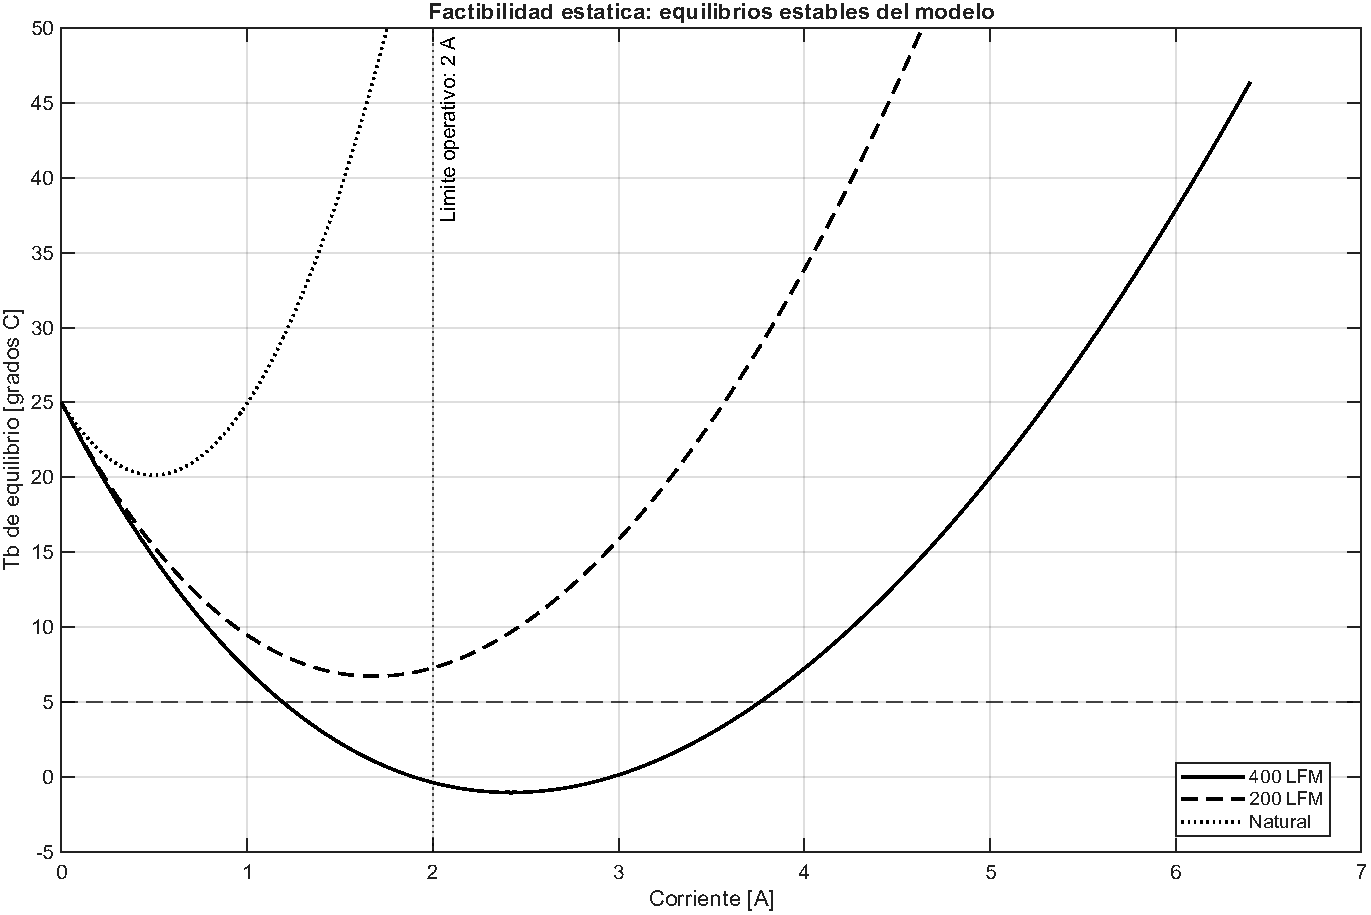
\includegraphics[width=\columnwidth]{factibilidad_termica.pdf}
\caption{Equilibrios del modelo para las tres condiciones de disipación. El barrido completo se distingue del límite operativo de 2 A. Fuente: ejecución recibida del grupo.}
\label{fig:factibilidad}
\end{figure}

\subsection{Revisión independiente del compensador recibido}\label{sec:revisionPI}
El archivo del integrante 2 entrega $K_c=0.75\,\mathrm{A/K}$ y $K_i=0.00645555\,\mathrm{A/(K\,s)}$. Para revisar esos parámetros sin cambiar el diseño se considera
\begin{equation}
C(s)=\frac{K_cs+K_i}{s},\qquad L_H(s)=-C(s)H(s)G(s).
\end{equation}
El controlador tiene un polo en el origen y un cero en $-K_i/K_c\simeq-0.0086074\,\mathrm{s^{-1}}$. Al incluir el estado de corriente y conservar los coeficientes del MAT, los polos de la transferencia cerrada sin reducción son aproximadamente
\begin{align}
 p_1&=-99.78052, &p_2&=-0.254673,\\
 p_3&=-0.0125240, &p_4&=-0.0086074,
\end{align}
en $\mathrm{s^{-1}}$. El modo nominal asociado con la cancelación estable se conserva en esta lista.

La comprobación algebraica independiente encuentra el cruce de ganancia en $\omega_c\simeq0.214175\,\mathrm{rad/s}$ y un margen de fase de $98.55^{\circ}$, definido en el cruce de magnitud unitaria \cite{mw_margin}. El valor ideal sin $H(s)$ era aproximadamente $98.68^{\circ}$. La diferencia es coherente con la pequeña fase adicional del estado de 10 ms a esa frecuencia.

Estos son resultados analíticos del modelo lineal obtenidos a partir de los coeficientes guardados; no son ensayos del PI en Simscape. El archivo \texttt{revisar\_compensador.m} permite contrastarlos mediante las herramientas de MATLAB, pero sus salidas no estaban guardadas en el RAR. No se concluye a partir de estos polos que el anti-windup o el arranque físico del PI estén validados.

\subsection{Sensibilidad y compromisos del sistema compensado}
\textit{PENDIENTE, integrante 1 con el modelo del integrante 3: repetir la sensibilidad con el PI, mantener ganancias y condiciones comunes y agregar la comparación con la Tabla~\ref{tab:sens}.}

\subsection{Compromisos de diseño}\label{sec:compromisos}
La ganancia $K_c$ concentra el principal compromiso del diseño. Un valor mayor acelera la respuesta y reduce el pico ante perturbaciones (Figura~\ref{fig:barrido}), pero exige más corriente, satura antes y amplifica el ruido de cuantización del sensor: cada paso de $0.0625\,\mathrm K$ produce un salto de $K_c\times0.0625\approx0.05\,\mathrm A$ en la corriente. El límite de $2\,\mathrm A$ también es un compromiso, porque protege el lazo contra la inversión de la ganancia a costa de no aprovechar toda la capacidad de enfriamiento de la celda.

La cancelación del polo lento hace que la respuesta a la referencia sea rápida ($158.6\,\mathrm s$ en la predicción ideal), pero deja ese polo en la respuesta a perturbaciones, que en el cálculo ideal tarda cerca de $300\,\mathrm s$ en volver a $\pm0.1\,\mathrm K$. Además, la cancelación depende de los parámetros: el polo de $-0.0086\,\mathrm{s^{-1}}$ cambia con la resistencia del disipador y con las masas, que siguen siendo provisionales. Si la cancelación no es exacta, aparece un par polo--cero cercano que agrega una cola lenta de poca amplitud, y exige recalcular los polos y el transitorio de la planta variada. La positividad de los coeficientes del modelo nominal no demuestra estabilidad para cualquier cambio térmico. La sensibilidad P se presenta en la Sección~\ref{sec:sensibilidad}; la comparación PI permanece pendiente.

El límite de $2\,\mathrm A$ se eligió con el disipador ventilado a $400\,\mathrm{LFM}$. Si el ventilador falla, el mínimo de la curva estática se desplaza a corrientes menores y queda por encima de $5\,^\circ\mathrm C$ (Tabla~\ref{tab:factibilidad}). En esos casos la referencia de $5\,^\circ\mathrm C$ es inalcanzable con cualquier controlador, el integrador lleva la corriente al límite y, en convección natural, el equilibrio calculado con $2\,\mathrm A$ queda cerca de $63\,^\circ\mathrm C$. Ese valor es distinto de la última muestra de la simulación de 1200 s, que todavía no alcanza el equilibrio. Por eso el sistema real necesita detectar la falla del ventilador, por ejemplo con la temperatura del lado caliente, y reducir la corriente. Como mejoras futuras se proponen una prealimentación de la temperatura ambiente para acelerar el rechazo de perturbaciones y un límite de corriente que dependa de la temperatura del lado caliente.


\textit{PENDIENTE, integrantes 2 y 3: cerrar el cumplimiento de especificaciones a partir de la simulación compensada y completar las mejoras de la implementación física.}

% ================================================================
% CONCLUSION P LISTA. COMPLETAR EL CIERRE DEL GRUPO.
% ================================================================
\section{Conclusiones}
El control P con sesgo nominal y corriente limitada a 2 A regula el arranque de la planta Simscape al entorno de 5 grados Celsius para las tres ganancias estudiadas. El fallo asociado con permitir 6.4 A no es una limitación inevitable del P: corresponde a operar fuera del intervalo útil nominal de la curva térmica.

Aumentar $K_p$ reduce el error ante un cambio de referencia y una carga constante, pero amplifica las fluctuaciones producidas por el ruido y aumenta la presencia de saturación. El arranque con error final casi nulo no elimina la limitación de error residual para referencias y cargas distintas del equilibrio nominal.

Los modelos lineal y físico conservan tendencias comunes, pero sus diferencias pueden cambiar la evaluación de una banda de desempeño: con $K_p=5$, la carga de 2 W deja 0.09524 K en la predicción lineal y 0.12285 K en Simscape. Además, la pérdida de disipación puede hacer imposible la referencia, independientemente de la ganancia del controlador.

La implementación utiliza una dinámica de corriente asumida de 10 ms y requiere que la futura comparación P/PI mantenga esa misma hipótesis. La ejecución recibida respalda la parte P en R2026a; la prueba final en R2025a, la simulación compensada y la integración del informe permanecen pendientes.

El diseño PI incorpora la acción integral para corregir el error estacionario de referencia y perturbación, con $K_c=0.75\,\mathrm{A/K}$, $T_i=116.2\,\mathrm s$ y anti-windup. Sus predicciones ideales y la comprobación auxiliar de Euler justifican contrastar esa propuesta con el P, pero no reemplazan los ensayos del modelo compensado. \textit{PENDIENTE, integrantes 2 y 3: cerrar la comparación y el cumplimiento final cuando se complete la validación exigida.}

% ================================================================
% REFERENCIAS EN ESTE MISMO ARCHIVO. AGREGAR LAS DE LOS COMPANEROS.
% ================================================================
\begin{thebibliography}{12}
\bibitem{hb} HB Corporation, \emph{Thermoelectric Cooler TEC1-12706}, rev. 2.03, pp. 1--3.
\bibitem{who_pqs} World Health Organization, \emph{WHO VAX IMD Terms \& Definitions, Master List 1.2, julio 2025}, definición de \emph{acceptable temperature range}. [En línea]. Disponible: \url{https://extranet.who.int/prequal/key-resources/documents/who-vax-imd-terms-definitions}. Consultado: nov. 2026.
\bibitem{ds18b20} Maxim Integrated (Analog Devices), \emph{DS18B20: Programmable Resolution 1-Wire Digital Thermometer}, hoja de datos. [En línea]. Disponible: \url{https://www.analog.com/media/en/technical-documentation/data-sheets/ds18b20.pdf}. Consultado: nov. 2026.
\bibitem{ogata} K. Ogata, \emph{Ingeniería de control moderna}, 5.ª ed. Madrid, España: Pearson Educación, 2010.
\bibitem{astrom} K. J. Åström y T. Hägglund, \emph{Advanced PID Control}. Research Triangle Park, NC, EE.\,UU.: ISA, 2006.
\bibitem{mw_pid} MathWorks, \emph{PID Controller}, Simulink. [En línea]. Disponible: \url{https://www.mathworks.com/help/simulink/slref/pidcontroller.html}. Consultado: nov. 2026.
\bibitem{mw_lim} MathWorks, ``Limitations,'' Simscape. [En línea]. Disponible: \url{https://www.mathworks.com/help/simscape/ug/limitations.html}. Consultado: nov. 2026.
\bibitem{mw_ss} MathWorks, ``State-Space,'' Simulink. [En línea]. Disponible: \url{https://www.mathworks.com/help/simulink/slref/statespace.html}. Consultado: nov. 2026.
\bibitem{mw_margin} MathWorks, ``margin,'' Control System Toolbox. [En línea]. Disponible: \url{https://www.mathworks.com/help/control/ref/dynamicsystem.margin.html}. Consultado: nov. 2026.
\end{thebibliography}

\end{document}
